\documentclass[conference]{IEEEtran}

\usepackage[numbers, sort, compress]{natbib}
\usepackage{graphicx}
\usepackage{amsmath}
\usepackage{amssymb}
\usepackage{color}
\usepackage{ifpdf}

\usepackage{dcolumn}
\usepackage{float}
\usepackage[utf8]{inputenc}
\usepackage{multirow}
\usepackage{rotating}

\usepackage[tight]{subfigure}



%\usepackage[numbers, sort, compress]{natbib}
%\usepackage{latex8}
%\usepackage{float}
%\usepackage{times}    
\usepackage{url}
\usepackage{listings}   
\usepackage{paralist}    
\usepackage{wrapfig}    
%\usepackage[small,it]{caption}
\usepackage{multirow}
\usepackage{ifpdf}
%\usepackage{srcltx}
%\usepackage{subfigure}
\usepackage{xspace}
\usepackage{keyval}  
\usepackage{color}

\definecolor{listinggray}{gray}{0.95}
\definecolor{darkgray}{gray}{0.7}
\definecolor{commentgreen}{rgb}{0, 0.4, 0}
\definecolor{darkblue}{rgb}{0, 0, 0.4}
\definecolor{middleblue}{rgb}{0, 0, 0.7}
\definecolor{darkred}{rgb}{0.4, 0, 0}
\definecolor{brown}{rgb}{0.5, 0.5, 0}

\usepackage[normalem]{ulem}
\makeatletter
\def\cyanuwave{\bgroup \markoverwith{\lower3.5\p@\hbox{\sixly \textcolor{cyan}{\char58}}}\ULon}
\def\reduwave{\bgroup \markoverwith{\lower3.5\p@\hbox{\sixly \textcolor{red}{\char58}}}\ULon}
\def\blueuwave{\bgroup \markoverwith{\lower3.5\p@\hbox{\sixly \textcolor{blue}{\char58}}}\ULon}
\font\sixly=lasy6 % does not re-load if already loaded, so no memory problem.
\makeatother

%!TEX root = sc12/pstar-sc2012-ieee.tex
\newif\ifdraft
%\drafttrue
\ifdraft
\newcommand{\onote}[1]{ {\textcolor{cyan} { (***Ole: #1) }}}
\newcommand{\terminology}[1]{ {\textcolor{red} {(Terminology used: \textbf{#1}) }}}
\newcommand{\owave}[1]{ {\cyanuwave{#1}}}
\newcommand{\jwave}[1]{ {\reduwave{#1}}}
\newcommand{\alwave}[1]{ {\blueuwave{#1}}}
\newcommand{\jhanote}[1]{ {\textcolor{red} { ***shantenu: #1 }}}
\newcommand{\alnote}[1]{ {\textcolor{blue} { ***andreL: #1 }}}
\newcommand{\amnote}[1]{ {\textcolor{blue} { ***andreM: #1 }}}
\newcommand{\smnote}[1]{ {\textcolor{brown} { ***sharath: #1 }}}
\newcommand{\msnote}[1]{ {\textcolor{cyan} { ***mark: #1 }}}
\newcommand{\note}[1]{ {\textcolor{magenta} { ***Note: #1 }}}
\else
\newcommand{\onote}[1]{}
\newcommand{\terminology}[1]{}
\newcommand{\owave}[1]{#1}
\newcommand{\jwave}[1]{#1}
\newcommand{\alnote}[1]{}
\newcommand{\amnote}[1]{}
\newcommand{\athotanote}[1]{}
\newcommand{\smnote}[1]{}
\newcommand{\jhanote}[1]{}
\newcommand{\msnote}[1]{}
\newcommand{\note}[1]{}
\fi

\newcommand{\pilot}{Pilot\xspace}
\newcommand{\pilots}{Pilots\xspace}
\newcommand{\pilotjob}{Pilot-Job\xspace}
\newcommand{\pilotjobs}{Pilot-Jobs\xspace}
\newcommand{\computeunit}{Compute Unit\xspace}
\newcommand{\computeunits}{Compute Units\xspace}
\newcommand{\cu}{CU\xspace}
\newcommand{\cus}{CUs\xspace}
\newcommand{\cs}{Compute Service\xspace}
\newcommand{\css}{Compute Services\xspace}
\newcommand{\pcs}{Pilot Compute Service\xspace}
\newcommand{\dataunit}{Data Unit\xspace}
\newcommand{\dataunits}{Data Unit\xspace}
\newcommand{\du}{DU\xspace}
\newcommand{\dus}{DUs\xspace}
\newcommand{\pilotdata}{Pilot-Data\xspace}
\newcommand{\pd}{PD\xspace}
\newcommand{\pds}{Pilot Data Service\xspace}
\newcommand{\pdss}{Pilot Data Services\xspace}
\newcommand{\su}{SU\xspace}
\newcommand{\sus}{SUs\xspace}
\newcommand{\schedulableunit}{Schedulable Unit\xspace}
\newcommand{\schedulableunits}{Schedulable Units\xspace}
\newcommand{\cc}{c\&c\xspace}
\newcommand{\CC}{C\&C\xspace}

\lstdefinestyle{myListing}{
  frame=single,   
  backgroundcolor=\color{listinggray},  
  %float=t,
  language=C,       
  basicstyle=\ttfamily \footnotesize,
  breakautoindent=true,
  breaklines=true
  tabsize=2,
  captionpos=b,  
  aboveskip=0em,
  belowskip=-2em,
  %numbers=left, 
  %numberstyle=\tiny
}      

\lstdefinestyle{myPythonListing}{
  frame=single,   
  backgroundcolor=\color{listinggray},  
  %float=t,
  language=Python,       
  basicstyle=\ttfamily \footnotesize,
  breakautoindent=true,
  breaklines=true
  tabsize=2,
  captionpos=b,  
  %numbers=left, 
  %numberstyle=\tiny
}

\newcommand{\up}{\vspace*{-1em}}
\newcommand{\upp}{\vspace*{-0.5em}}
\newcommand{\numrep}{8 }
\newcommand{\samplenum}{4 }
\newcommand{\tmax}{$T_{max}$ }
\newcommand{\tc}{$T_{C}$ }
\newcommand{\tcnsp}{$T_{C}$}
\newcommand{\bj}{BigJob}

%  \setlength{\parskip}{0.05ex} % 1ex plus 0.5ex minus 0.2ex}
%  \setlength{\parsep}{0pt}
%  %\setlength{\headsep}{0pt}
%  \setlength{\topskip}{0pt}
%  \setlength{\topmargin}{0pt}
%  %\setlength{\topsep}{0pt}
%  \setlength{\partopsep}{0pt}

% This is now the recommended way for checking for PDFLaTeX:


\ifpdf
\DeclareGraphicsExtensions{.pdf, .jpg, .tif}
\else
\DeclareGraphicsExtensions{.eps, .jpg}
\fi

\tolerance=1000
\hyphenpenalty=10


\begin{document}
%\conferenceinfo{WOODSTOCK}{'97 El Paso, Texas USA}
% \conferenceinfo{ECMLS'11,} {June 8, 2011, San Jose, California, USA.}
% \CopyrightYear{2011}
% \crdata{978-1-4503-0702-4/11/06}
% \clubpenalty=10000
% \widowpenalty = 10000

\title{P*: A Model of Pilot-Abstractions}

\author{
  Andre Luckow$^{1}$, Mark Santcroos$^{2,1}$, Ole Weidner$^{1}$, Andre Merzky$^{1}$, Pradeep Mantha$^{1}$, Shantenu Jha$^{3,1*}$\\[0.4em]
  \small{\emph{$^{1}$Center for Computation \& Technology, Louisiana State University, USA}}\\[-0em]
  \small{\emph{$^{2}$Bioinformatics Laboratory, Academic Medical Center, University of Amsterdam, The Netherlands}}\\[-0em]
  \small{\emph{$^{3}$ Rutgers University, Piscataway, NJ 08854, USA}}\\[-0em]
%  \small{\emph{$^{4}$ School of Informatics, University of Edinburgh, UK }}\\[-0.3em]
  \small{\emph{$^{*}$Contact Author: \texttt{shantenu.jha@rutgers.edu}}}\\[-0.3em]
  \up\up}

\date{}
\maketitle

\begin{abstract} 

 % Distributed cyberinfrastructures (CI) and applications require the
  % ability to determine and utilize resource
  % selection\alnote{selection somehow does not fit} at runtime
  % (dynamically), and not just before execution (statically).
  % they have been utilized on many production distributed
  % cyberinfrastructures.  they have been notable in their ability to
  %\alnote{the following sentence is just a fragement}

  \pilotjobs support effective distributed resource utilization, and
  are arguably one of the most widely-used distributed computing
  abstractions -- as measured by the number and types of applications
  that use them, as well as the number of production distributed
  cyberinfrastructures that support them.  In spite of broad uptake,
  there does not exist a well defined, unifying conceptual model of
  \pilotjobs which can be used to define, compare and contrast
  different implementations.  Often \pilotjob implementations are
  strongly coupled to the distributed cyberinfrastructure they were
  originally designed for. 
  % there exist multiple distinct and incompatible implementations of
  % pilot-jobs.
  These factors present a barrier to extensibility and
  interoperability. This paper is an attempt to (i) provide a minimal
  but complete model (P*) of \pilotjobs, (ii) establish the generality
  of the P* Model by mapping various existing and well known \pilotjob
  frameworks such as Condor and DIANE to P*, (iii) derive an
  interoperable and extensible API for the P* Model (Pilot-API), (iv)
  validate the implementation of the Pilot-API by concurrently using
  multiple distinct pilot-job frameworks on distinct production
  distributed cyberinfrastructures, and (v) apply the P* Model to
  \pilotdata.
\end{abstract}
%\category{H.4}{Information Systems Applications}{Miscellaneous}
%terms{Theory}
%\keywords{ACM proceedings, \LaTeX, text tagging}
%\up\up

%and are usable on different infrastructures

\section{Introduction and Overview} 

The seamless uptake of distributed infrastructures by scientific
applications has been limited by the lack of pervasive and
simple-to-use abstractions at multiple levels -- at the development,
deployment and execution stages~\cite{dpagrid2009}.  Even where meaningful abstractions
exist, the challenges of implementing them in an extensible, reliable
and scalable manner, so as to support multiple applications are
formidable.  The lack of appropriate implementations has in fact
resulted in ``one-off'' solutions that address challenges in a highly
customized manner.  Tools and implementations are often highly
dependent on and tuned to a specific execution environment, further
impacting portability, reusability and extensibility.  Semantic and
interface incompatibility are certainly barriers, but so is the lack
of a common architecture and conceptual framework upon which to
develop similar tools a barrier.  This general state of affairs also
captures the specific state of the abstractions provided by {\it
  \pilotjobs (PJ)}.  There are a plethora of working definitions and
roles for \pilotjobs; from our perspective, a \pilotjob provides the
ability to utilize a placeholder job as a container for a dynamically
determined set of compute tasks.

%reinforces the fragmentation~\cite{dpa_surveypaper}.
% there remains, scope for improvement in both the range and number of
% supported abstractions and the type of infrastructure over which such
% abstractions are made available.

Distributed cyber/e-infrastructure is by definition comprised of a set
of resources that is fluctuating -- growing, shrinking, changing in
load and capability (in contrast to a static resource utilization
model of traditional parallel and cluster computing systems).  The
ability to utilize a dynamic resource pool is thus an important
attribute of any application that needs to utilize distributed
cyberinfrastructure (DCI) efficiently. As a consequence of providing a
simple approach for decoupling workload management and resource
assignment/scheduling, PJ provide an effective abstraction for dynamic
execution and resource utilization in a distributed context.  Not
surprisingly, \pilotjobs have been one of the most successful
abstractions in distributed computing.  The fundamental reason for the
success of the \pilotjob abstraction is that \pilotjobs liberate
applications/users from the challenging requirement of mapping
specific tasks onto explicit heterogeneous and dynamic resource pools.
\pilotjobs thus shield applications from having to load-balance tasks
across such resources.  The \pilotjob abstraction is also a promising
route to address specific requirements of distributed scientific
applications, such as coupled-execution and application-level
scheduling~\cite{ko-efficient,DBLP:conf/hpdc/KimHMAJ10}.


A variety of PJ frameworks have emerged: Condor-G/
Glide-in~\cite{condor-g}, Swift~\cite{Wilde2011},
DIANE~\cite{Moscicki:908910}, DIRAC~\cite{1742-6596-219-6-062049},
PanDA~\cite{1742-6596-219-6-062041}, ToPoS~\cite{topos},
Nimrod/G~\cite{10.1109/HPC.2000.846563}, Falkon~\cite{1362680} and
MyCluster~\cite{1652061}, to name a few. Although they are all, for
the most parts, functionally equivalent -- they support the decoupling
of workload submission from resource assignment -- it is often
impossible to use them interoperably, or even just to compare them
functionally or qualitatively.
% The situation is reminiscent of the
% proliferation of functionally similar yet incompatible workflow
% systems, where in spite of significant a posteriori effort on workflow
% system extensibility and interoperability (thus providing post-facto
% justification of its needs), these objectives remains difficult if not
% infeasible.
% \pmnote{ The last statement is a little complex to
%   understand, can it be more simple,since i think its main point which
%   explains why we need interoperable-API }

%Where effective abstractions exist a problem in the 
%The general problem applies to the specific situation of pilot-jobs.

%Different projects and users have rolled-out their own PJ
%abstractions.  

% The fact that users have voted with their feet for PJs reinforces that
% the PJ abstraction is both a useful and correct abstraction for
% distributed CI; 

% the fact that it has become an ``unregulated cottage
% industry'' reaffirms the lack of common nomenclature, integration,
% interoperability and extension, and poses barriers to extensibility and
% interoperability as a consequence. 


% Also, maybe interoperability isnt what is desired, but reusability
% and or ease of customisation.  Talk about analogy with workflow
% systems.  Interestingly there exist many implementations of the PJ
% abstraction, wherein d

% Interestingly there exist many implementations of the PJ abstraction,
% wherein different projects and users have rolled-out their own. The
% fact that users have voted with their feet for PJs reinforces that the
% Pilot-Job is both a useful and correct abstraction for distributed CI;
% the fact that it has become an ``unregulated cottage industry''
% reaffirms the lack of common nomenclature, integration,
% interoperability and extension.


% In \S{III} we introduce TROY -- A Tiered Resource OverlaY -- as an
% implementation of the P* Model. TROY provides an API for the P* Model
% and exposes the semantics of PJ frameworks; TROY also has a runtime
% system that enables it to work with different middleware on
% heterogeneous distributed platforms.

% Implementations of PJ frameworks, such as BigJob and DIANE, are
% integrated into TROY via an adaptor mechanism; we posit that the TROY
% framework and API can be used for most, if not all PJ frameworks.

% The P* Model captures the essence of most, if not all existing PJ
% frameworks.

Our objective is to provide a minimal, but complete model for \pilot
abstractions~\cite{pstar-2012} -- referred to as P* Model ("P-star"),
which we present in \S\ref{sec:pilot-model}.  We also investigate
generalizations to the base P* Model.  A natural and logical extension
of the P* Model arises from the opportunity to extend it to include
data in addition to computational tasks. This leads to analogous
abstraction to the \pilotjob: the \emph{\pilotdata (PD)}
abstraction. The potentially consistent treatment of data and compute
suggests symmetrical compute and data elements in the model; thus we
refer to this model as the P* Model of Pilot Abstractions.

The P* Model provides a conceptual basis to compare and contrast
different PJ frameworks -- which to the best of our knowledge is the
first such attempt. In \S\ref{sec:pilot-model}, we also apply the P*
Model to data and introduce {\it Pilot-Data} as an abstraction 
that is analogous \pilotjobs. In \S\ref{sec:pilot-job-frameworks}
we validate the P* Model by analyzing well-known PJ frameworks
(BigJob, Condor-G/Glide-in, DIANE) and mapping them to the elements of
the P* Model.\pmnote{ analyzation of tools present, but validation, i dont think we did, since we dont have any experiments} \S\ref{sec:pilot-api} of this paper motivates and
describes the Pilot-API; we discuss how existing and widely used
\pilotjob frameworks can be used through the
Pilot-API. \S\ref{sec:exp_res} describes the experiments and
performance measurements used to characterize the workings of the
Pilot-API and to demonstrate interoperability across middleware,
platform and different PJ frameworks. To further substantiate the
impact of P*, we will demonstrate interoperability between different
PJ frameworks. %BigJob and DIANE.
We believe this is also the first demonstration of concurrent
interoperation of different \pilotjob implementations. Performance
advantages arising from the ability to distribute part of a
data-intensive workload are discussed; interoperable capabilities
increase flexibility in resource selection and optimization.

It is worth noting that \pilotjobs are used on every major national
and international DCI, including NSF/XSEDE, NSF/DOE Open Science Grid,
EU EGI and others; they are used to support hundreds and thousands of
tasks daily. Thus we believe the impact and validation of this paper
lies in its ability to not only influence but also bridge the theory
and practice of \pilotjobs, and thus multiple domains of science
dependent on distributed cyberinfrastructure.

% After validating the P* Model -- as measured by extensibility and
% interoperability -- 
%Before discussing the P* Model, 

%  which is also partly motivated by
% the status of the usage and availability of the pilot abstraction
% vis-\`{a}-vis the current landscape of distributed applications and
% cyberinfrastructure.

 % Collectively pilot-jobs support
% hundreds of thousands if not millions of tasks every day.  As we will
% show, the Pilot-API provides a single uniform API to PJ-frameworks
% thus providing for the first time... removing barriers to...
% \jhanote{fix..}

\note{Reviewer Comment: Is this really the first work of its kind? Are
  there no other related attempts?}

% All pilot-job frameworks (whether they adhere rigorously to the P*
% model or not), have these {\it elements}, but differ in {\it
%   characteristics}.  specific attributes \alnote{What would be an
%   attribute in this context?} and Further, we will show that these
% elements and interactions can be used to describe a pilot-data
% model.

\section{The P* Model of Pilot-\\Abstractions}
\label{sec:pilot-model}

An initial motivation for the P* Model of pilot-abstractions is to
provide a common analytical framework to understand commonly
used \pilotjob frameworks.  The P* model was derived by analysing many
\pilotjob implementations.  We first present
the common {\it elements} of the P* Model, followed by a description
of the {\it characteristics} that determine the interaction of these
elements and the overall functioning of any \pilotjob framework 
consistent with the P* Model.  

Before we proceed to discuss the P* Model, it is important to
emphasize that there exists a plethora of terms (abstraction,
model, framework, implementation etc) that are overloaded and
overlapping, and often used inconsistently in the literature;
thus we establish context and usage of relevant terms.

% \amnote{The previous paragraph seems to indicate that we'll define ''abstraction,
% model, framework, and implementation'' - but we don't.}

\B{\I{Terms and Usage:}} A \pilotjob can be defined as an \emph{
  abstraction} that generalizes the reoccurring concept of utilizing a
placeholder job as a container for a set of compute tasks; an instance
of that placeholder job is commonly referred to as \emph{\pilotjob}
or \emph{pilot}. The P* \emph{model} provides a % specific,
comprehensive description of the \pilotjob abstraction, based on a set of
identified elements and their interactions. The P* Model can be used
as a {\it conceptual model}, for analyzing different implementations
of the \pilotjob abstraction. The \emph{Pilot-API} provides an
interface that exposes a sub-set of the P* elements and
characteristics to applications.  It is important to distinguish P* --
which provides a conceptual (abstract) model, from an implementation
of the P* Model. A \emph{\pilotjob framework} refers to a specific
instance of a \pilotjob implementation
that provides the complete \pilotjob functionality (e.\,g.\
BigJob and DIANE).

%\alnote{The next sentence is not really helpful - we also not really
%  using the term PJ system in the rest of the paper:} The term
%"pilot-job system" could have been used as well, but past experience
%shows that even with ``system'', there remains scope for confusion
%between the pilot-job itself and associated infrastructure (e.g, the
%literature abounds with inconsistent usage of the term ``workflow
%systems'').

% \jhanote{\emph{Other Terms:} Resource-Manager and agent..}
% \jhanote{This could be a good place to describe (not define) an 

\begin{figure}[t]
    \centering
    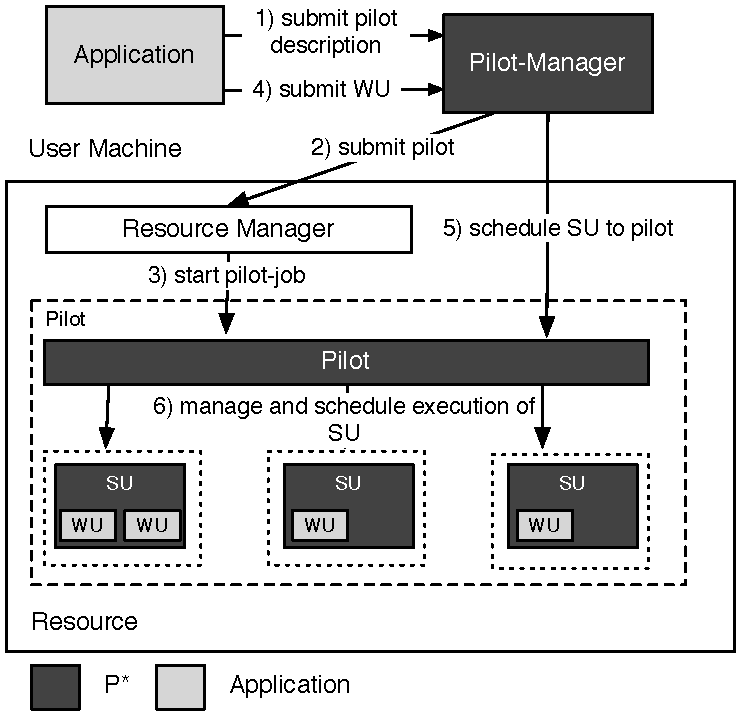
\includegraphics[width=0.48\textwidth]{../figures/pstar_model_single.pdf}
    \caption{\I{\textbf{P* Model: Elements, Characteristics and
        Interactions:} The manager has two functions: it manages 1)
      Pilots (step 1-3) and 2) the execution of \cus. After a \cu is
      submitted to the manager, it transitions to an \su, which is
      scheduled to a \pilot by the PM. The \pilot then schedules the
      \su to an available resource.}\up\up}
    \label{fig:figures_pstar}
\end{figure}

% and is responsible for the execution of \alwave{SUs/tasks}
% onto the resource.

  % \alnote{\textbf{The RM assigns a slice of the Resource to the
  %     pilot -- that pilot then acts as RM for that resource slice.}
  %   I think simply equating a pilot with a RM is bit too
  %   simplistic. In a sense it is a application-level resource
  %   manger. Not sure what to do}

%\input{sectionII_comments}
%\alnote{use pilot NOT pilot-job}
% via the resource's RM system. 

\noindent 
\subsection{Elements of the P* Model}

\noindent This sub-section defines the elements of the P* Model:

\noindent$\bullet$ \textbf{\pilot (Pilot-Compute):} The \pilot is the
entity that actually gets submitted and scheduled on a resource.  The
Pilot provides
application (user) level control and management of the set of
allocated resources.

% \amnote{So, we are still using 'Pilot-Compute' instead of 'Compute-Pilot'?  Note
% that we agreed for the Pilot API to switch to ComputePilot (CP)}
% \alnote{I am not aware of such an agreement. The Pilot-API uses Pilot-Compute (see link provided). We definitely should not focus on naming wars in the last
% 10 h.}
% \amnote{There is 'Compute Unit' (space), but Pilot-Compute (dash).  Well, we
%     have two of each type, so at least we are not favoring any version ;-)}

\noindent$\bullet$ \textbf{\computeunit  (\cu):} A \cu  encapsulates a 
  self-contained piece of work (a compute task) specified by the application, that is
  submitted to the \pilotjob framework. There is no intrinsic notion
  of resource associated with a \cu.

\noindent$\bullet$ \textbf{Scheduling Unit (SU):} SUs are the units of 
  scheduling, internal to the P* Model, i.e., it is not known by or
  visible to an application. Once a \cu is
  under the control of the \pilotjob framework, it is assigned
  to an SU.
  % An SU is created after the submission of
  %   a \cu, i.\,e.\ once a \cu \ has been passed into the control of the
  %   pilot-job framework. 
%  \jhanote{Could we say: Once a \cu has been
%    passed into the control of the pilot-job framework, it is assigned
%    to an SU} \alnote{sounds good. done.}

\noindent$\bullet$ \textbf{Pilot-Manager (PM):} The PM is responsible for (i)
  orchestrating the interaction between the \pilots as well as the
  different components of the P* Model (\cus, \sus) and (ii) decisions
  related to internal resource assignment (once resources have been
  acquired by the \pilotjob).  For example, an SU can consists of one
  or more \cus. Further, \cus and \sus can be combined and aggregated;
  the PM determines how to group them, when \sus are scheduled and
  executed on a resource via the \pilot, as well as how many resources
  to assign to an SU.

  \amnote{to (i): it is not clear at this point why there should be interactions
    between pilots.}


% the different characteristics of the P* model. It
%   facilitates the coordination between the different P* elements,
%   i.\,e.\ the pilots, \cus and SUs. 
% A PM can e.\,g.\ manage solely one
%   or multiple pilots.

%   For example, the PM has the flexibility to combine and schedule \cus,
%   e.\,g.\ it can determine when a \cu is run and what as well as how
%   many resources it will receive.


% The application itself is not strictly part of the core P* Model.
% The term application generally refers to the upper layer of the
% stack.

  
  The application utilizes a PJ framework to execute multiple
  instances (ensemble) of an application kernel (kernel: 
  the actual binary that gets executed), or
  alternatively instances of multiple different application kernels (a
  workflow).  To execute an application kernel, an application must
  define a \cu specifying the application kernel as well as other
  parameters. This \cu is then submitted to the PM (the entry point to
  the \pilotjob framework), where it transitions to an \su. The PM is
  then responsible for scheduling the \su onto a \pilot and then onto
  a physical resource.  As we will see in
  \S\ref{sec:pilot-job-frameworks}, the above elements can be mapped
  to specific entities in many existing \pilotjob frameworks --
  more than one logical element are often rolled into
  one specific entity in a \pilotjob.

% \textbf{Diane Definition of Terms: } The computation consists of
% many worker processes which communicate with one master process (the
% worker processes do not need to share the filesystem nor
% memory). The ensemble of computation is called a run and it consists
% of many tasks which may be executed in parallel. A task is defined
% as a set of parameters which are produced by the RunMaster (running
% on a master node) and consumed by the WorkerAgent (running on a
% worker node).
% 
% from 
% 
% DIANE assumes the master-worker computing model (Fig.
% 1). Client sends job parameters to the Planner which partitions
% the job into smaller tasks executed by the Workers. Integrator
% is responsible for merging the results of task execution and
% sending the final job outcome to the Client.


\subsection{Characteristics of P* Model}
\label{sec:p_star_elements}

%\jhanote{Why not have Binding as the first characteristics?}

% To understand % the degrees of freedom that any specific pilot-job
% % implementation must constraint as well as
% the functioning of
% pilot-jobs implementation, 
%These characteristics are integral components of the P* Model, in
% Further, these properties are important for the implementation of
% P*.  list several characteristics.
% The way the coordination between the different elements
% is handled is required to understand a PJ implementation.
 
We propose a set of fundamental properties/characteristics that
describe the interactions between the elements, and thus aid in the
description of P* Model.

% \alnote{ok} \jhanote{One strategy could be to not define the different
%   types, but just list/enumerate? Akin to Communication. i.e. explain
%   what coordination is for, what is being coordinated, how (the 3
%   types)}

\textbf{Coordination Characteristics:} these describe how
various elements of the P* Model, i.\,e.\ the PM, the \pilot, the \cus
and the SUs, interact. A common coordination pattern is master/worker
(M/W): the PM represents the master process that controls a set of
worker processes, the \pilots. The point of decision making is the
master process. In addition to the \emph{centralized} M/W, M/W can
also be deployed \emph{hierarchically}.  Alternatively, coordination
between the elements, in particular the \pilots, can be performed so as
to be \emph{decentralized}, i.\,e.\ without central decision making
point.

%\input{sectionIII-comments}

\textbf{Communication Characteristics:} The communication characteristics describes the
mechanisms for data exchange between the elements of the P* Model:
e.\,g.\ messages (point-to-point, all-to-all, one-to-all, all-to-one,
or group-to-group), streams (potentially unicast or multicast),
publish/subscribe messaging or shared data spaces.
		
\textbf{Scheduling Characteristics:} these describe the
process of mapping a \su to resources via a \pilot, and potential
multiple levels of scheduling. Scheduling has a spatial component
(which \su is executed on which \pilot?) but also a temporal component
(when to bind?). The different scheduling decisions that need to be
made are representative of multi-level scheduling decisions that are
often required in distributed environments.  For example, for the
temporal component: a \su can be bound to a \pilot either before
the \pilot has in turn been scheduled ({\it early} binding), or 
binding occurs if the \su is bound after the \pilot has been
scheduled ({\it late} binding).  
% In general, there are multiple-levels at which scheduling
% decisions, i.e., resource selection and binding, are made.

The term {\it agent}, although not a part of the P* Model, finds
mention when discussing implementations. For the purposes of this
paper, an agent refers to a ``proxy process'' 
% that either % inside the % pilot-job framework
that has some decision making capability, and could aid the
implementation of one or more of the characteristics of the P* Model
(coordination, communication, scheduling), within a \pilotjob
framework.  These agents can be used to enforce a set of
(user-defined) policies (e.g.  resource capabilities, data/compute
affinities, etc.) and heuristics.




\subsection{P* as a Model for Pilot-Data}
\label{sec:pilot-data}
% \alnote{Should we merge this with section 2... At least we need to
%   move it before the performance section}

% \jhanote{Yes, and we need to supplement it. Maybe cut-n-paste from
%   architecture / flow from the MR paper for the meantime?}

\note{Reviewer Comment: Perhaps the most interesting component of the research 
is the generalization of the model to data, beyond computing jobs. This 
portion of the research could probably benefit from being expanded.}


Many scientific applications have immense data requirements, which are
projected to increase dramatically in the near future~\cite{hey2009}. 
%The small genome alignment tool scenario e.\,g.\ operates on a input data set 
%of $1.9$\,GB per \cu. 
While \pilotjobs efficiently support late-binding of
\I{\computeunits} and resources, the analogous management of data in
distributed systems remains a challenge due to various reasons: (i) the
placement of data is often decoupled from the placement of Compute Units and
Pilots, i.\,e.\ the application must often manually stage in and out its data
using simple scripts; (ii) heterogeneity, e.\,g.\ with respect to storage,
filesystem types and paths, often prohibits or at least complicates late
binding decisions; (iii) higher-level abstraction that allow applications to
specify their data dependencies on an abstract, logical level (rather than on
file basis) are not available; (iv) due to lack of a common treatment for
compute and data, optimizations of data/compute placements are often not
possible.
% For example, in scenario (B3) and (B4) presented in
% section~\ref{sec:fg-xsede-osg-egi}, even though the 50\,\% of the
% input data set is shared for all \cus, the complete data is staged for
% each \cu.

In addition, applications must cope with various other challenging,
data-related issues, e.\,g.\ varying data sources (such as sensors
and/or other application components), fluctuating data rates, transfer
failures, optimizations for different queries, data-/compute
co-location etc. While these issues can be in principal handled in an
application-specific way, the usage of higher-level abstractions, such
as a common \pilot-based abstraction for compute and data is
preferable.  

% Thus, having defined the P* model, we explore its extension to data.

This motivates an analogous abstraction that we call \emph{\pilotdata
  (PD)}. \jwave{PD provides late-binding capabilities for data by
  separating the allocation of physical storage and application-level
  data units.} Further, it provides an abstraction for expressing and
managing relationships between data units and/or compute units. These
relationships are referred to as \emph{affinities}.

% \jhanote{difficult to use affinity without defining it..}
% \alnote{tried to describe affinities a little bit better}

%\alnote{Extension vs. Application vs. Translation}
\subsubsection*{P* Model Elements for Data}

% A Pilot-Data Framework facilitates the late-binding between data units
% and physical storage resources, the so called pilot-stores.

The elements defined by P* can be extended with the following elements:

%\alnote{What is the role of SU in Data?}

\noindent$\bullet$
  \textbf{\pilot (Pilot-Data):} A \pilotdata (\pd) functions as a 
	placeholder object that reserves the space
	for data units. PD facilitates the late-binding of data and resource and is
	equivalent to the \pilot in the compute model.

\noindent$\bullet$
  \textbf{Data Unit (DU):} DU is the base unit of data assigned by
  the application,  e.\,g.\ a set of data files. 
%Multiple DUs can be aggregated    within a Data Unit Set.

% \noindent$\bullet$ \textbf{Pilot-Data (PD):} PD allows the logical grouping of DUs
%   and the expression of data-data affinities. This collection of files
%   can be associated with an extensible set of properties. One of these
%   properties is affinity. 

\noindent$\bullet$
  \textbf{Scheduling Unit (\su):} is an internal unit of scheduling (as in 
  the compute case). The Pilot framework can aggregate or split DUs into one 
  or more SUs.

\noindent$\bullet$ 
  The \textbf{Pilot-Manager (PM)} is the same as in the compute model and
  implements the different characteristics of the P* Model. It is responsible for
  managing \dus and \sus. Data is submitted to the framework via the PM. The PM
  which is responsible for mapping \dus to \sus and for conducting decision 
  regarding resource assignments. \sus are placed on physical resources via the \pilot.

Note, each element can be mapped to an element in the P* Model by
symmetry, e.\,g., a DU correspond to a \cu  in the original P* Model; 
a PD is a placeholder reserving a certain amount of storage on a physical 
resource and corresponds to the \pilot in the P* Model.

% \jhanote{PJ Model is confusing. Either it is P Model or PJ
%   Framework} \alnote{ok}

% A particular critical requirement for data-intensive application, is
% the management of affinity between DUs and also between \cus and
% DUs. Thus, Pilot-Data introduces the PD container object for
% expressing relationships between DUs. A PD corresponds to an SU in
% the \jwave{PJ model}, i.\,e.\ it is used as scheduling unit for
% internal optimizations, e.\,g.\ the grouping of DUs. Having
% instantiated a PD, it can be assigned to a PS via the PD manager. A
% PS is a placeholder reserving a certain amount of storage, i.\,e.\
% it corresponds to a pilot in the pilot-job model. By associating a
% PD to a PS the data is actually moved to the physical location
% associated with the PS. The PD manager facilitates the creation of
% PSs, schedules data movements (with respect to specified affinities)
% and manages data accesses.

\subsubsection*{P* Model Characteristics for Data}

While the extended P* Model introduces new elements, the
characteristics however, remain the same to a great extent. The
coordination characteristic describes how the elements of PD interact,
e.\,g.\ utilizing the M/W model; the communication characteristic can
be applied similarly. The scheduling characteristics must be extended
to not only meet compute requirements, but also to support common data
patterns. The scheduling component particularly needs to consider
affinities, i.\,e.\ user-defined relationships between \cus and/or
\dus. Data-data affinities e.\,g.\ exist if different \dus must be
present at the same resource; data-compute affinities arise if
data and compute must be co-located -- if their
current location is different, data and compute placement decisions
are made by the scheduler based on defined policies, affinities and
dynamic resource information.


\subsection{Putting it all together} 

Figure~\ref{fig:figures_pstar} illustrates the interactions between the
elements of the P* Model.  The figure focuses on Pilot-Compute, for
simplicity, but immediately applies to Pilot-Data by symmetry.  First, the
application specifies the capabilities of the required resources using a
\pilotjob description (step 1). The PM then submits the necessary number of
\pilots to fulfill the resource requirements of the application (step~2). Each
\pilot is queued at a resource manager, which is responsible for starting
the \pilot (step~3). There can be variations of this flow: while in the
described model, the application defines the required resources, the PM could
also decide based on the submitted \cu \ workload whether and when it submits
new \pilots.

%\jhanote{What about the Resource Manager? Is it part of the resource}

The application can submit \cus to the PM at any time (step~4). A submitted
\cu \ becomes an \su, i.\,e.\ the PM is now in control of its scheduling. In
the simplest case one \cu \ corresponds to one \su; however, SUs can be
combined and aggregated to optimize throughputs and response times. Commonly,
a hierarchical M/W model for coordination is internally used: the PM uses M/W
to coordinate a set of \pilots, the \pilot itself acts as manager for the
execution of the assigned SUs.

Scheduling decisions can be made on multiple levels. A \pilot is bound
to a physical resource on which it is responsible for a particular
resource set. The PM is responsible for selecting a \pilot for an \su
(step 5). Once a \su has been scheduled to a \pilot, the \pilot decides
when and on which part of the resource an \su is executed.  Further,
the \pilot manages the subsequent execution of an \su (step~6).  There
can be variations of this flow.  PJ frameworks with decentralized
decision making e.\,g.\ often utilize autonomic agents that % accept
% respectively
pull SUs according to a set of defined policies.

% \jhanote{Isn't
%   the pilot already bound to a specific resource? Or isn't the pilot
%   bound to a resource and thereby the \su bound to a resource
%   indirectly, and not directly?}  \alnote{Yes, the pilot is bound to a
%   specific resource set, assigning a \su to a pilot means that it can
%   be executed somewhere on this resource set. The pilot decides on
%   which node a \su is run. There can be trivial cases, e.g. DIANE where
%   this decision making does not exist: 1 worker agent == 1 core == 1
%   task. Should we make this more explicit?} \jhanote{Yes -- we
%   could/should make more explicit the fact that pilot is already bound
%   to a resources and assigning a \su to a pilot means it can be
%   executed anywhere on this resource set.} \alnote{refined}
% The above description presents a
% typical example of the inner working of a PJ framework, but alternative
% implementation of the P* characteristics are possible. 


%\alnote{TODO: add paragraph on Pilot-Data}

\note{Reviewer Comment:  For instance, utilities such as GLexec which have 
been developed so that the security model is preserved between the execution 
of the \su and the CU should be part of P* and appear somewhere in Figure 1.}

\note{Reviewer Comment: As the name suggest, the Pilot Job concept is
  very computation oriented and how to make the model evolve towards a
  solution which would be able to take into account application data
  requirements is an open question. Authors actually identifies this
  issue as Section 6 is devoted to an abstraction for
  Pilot-Data. However, the Pilot-Data API, which more or less mimics
  the PilotJob API is not very convincing in the sense that the
  interaction between the 2 APIs are not discussed at all. Maybe
  Pilot-Data should be presented as part of the P* model and section 6
  should be dedicated to the implementation of the 2 APIs to
  data-intense computing.}

\section{Pilot-Job Frameworks}

\label{sec:pilot-job-frameworks}

\note{Reviewer Comment: The analyze of coordination in PJ framework is very 
focused and not exhaustive enough in terms of frameworks investigated. Thus 
it's difficult to draw general conclusion. It would have been perhaps better 
to have an analytical model of P* which identifies the major components of the 
performance and compares this analysis with experimental measurements.}

\note{Reviewer Comment: What about other frameworks? Can they be incorporated? 
Why were these particular ones selected?}

% \note{OW says: we have this obsession with the term 'framework', but
%   not everything is a framework, e.g., while BigJob and DIANE somewhat
%   resemble a framework, I do not see how Condor can qualify as one.\\
%   For now, I changed the title to 'systems'. If there are no
%   objections, I will make this consistent throughout the
%   text}\alnote{I think we should keep frameworks, I do not see why
%   Condor is not a framework - we also would break consistency with our
%   terms and definitions in section II.}\note{OW says: "In computer
%   programming, a software framework is an abstraction in which
%   software providing generic functionality can be selectively changed
%   by user code, thus providing application specific software." This is
%   definetely not the case for Condor and not really for BigJob. DIANE
%   somewhat resembles a framework.}  \note{OW says: What if we call it
%   Pilot-Job Implementations}

% As more applications take advantage of dynamic execution, the
% Pilot-Job concept has grown in popularity and has been extensively
% researched and implemented for different usage scenarios and
% infrastructure.  \jhanote{The previous sentence is a repeat of one of
%   the high-level motivations of this work. I propose we
%   remove}\alnote{ok}

The aim of this section is to provide a basic understanding of some of
the most commonly used PJ frameworks. This will serve to both
motivate the development of the P* Model as well as validate it.  In
particular, we focus on Condor-G/Glide-in, BigJob and DIANE, and show
that the P* Model can be used to explain/understand these and
other PJ frameworks.

%There is a variety of PJ implementations:
%Condor-G/Glide-in~\cite{condor-g}, Swift~\cite{Wilde2011},
%DIANE~\cite{Moscicki:908910}, DIRAC~\cite{1742-6596-219-6-062049},
%PanDA~\cite{1742-6596-219-6-062041}, ToPoS~\cite{topos},
%Nimrod/G~\cite{10.1109/HPC.2000.846563}, Falkon~\cite{1362680} and
%MyCluster~\cite{1652061}.

%\jhanote{The aim of this section is to provide a conceptual validation
%  of the P* model by describing/explaining the most commonly used
%  PJ-frameworks and showing how the individual PJ-frameworks map to
%  the P* model, i.e., can be explained by the P* model}

\begin{figure}[t]
	\up\up\up
	\centering
	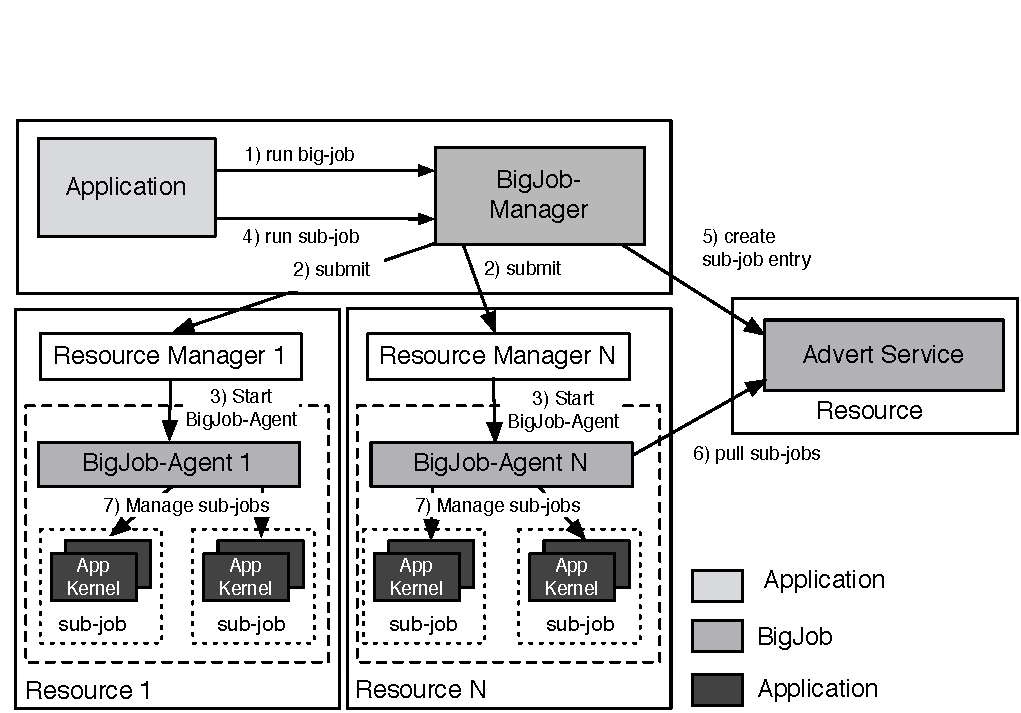
\includegraphics[width=0.48\textwidth]{../figures/re_bigjob_interactions.pdf}
	\caption{\I{\textbf{BigJob Architecture and Mapping to P*:}} The
          BJ architecture resembles many elements of the P* Model. The
          BigJob-Manager is the central Pilot-Manager, which
          orchestrates a set of \pilots. Each \pilot is represented by a
          decentral component referred to as the BigJob-Agent. Sub-job
          -- the \cus -- are submitted via the PM. \cus are mapped 1:1
          to \sus.\up\up}
	\label{fig:figures_re_bigjob_interactions}
	%\up
\end{figure}



\subsection{Condor-G/Glide-in}

The Condor project pioneered the concept of Pilot-Jobs by introducing the
\textit{Condor-G/Glide-in} mechanisms~\cite{condor-g} which allow the
temporary addition of Globus GRAM controlled HPC resources to a Condor
resource pool. The \pilot is exposed as a complete Condor
pool that is started via the Globus GRAM service of a resource. This mechanism
is referred to as Condor Glide-in. Subsequently, jobs (CUs) can be submitted
to the Condor Glide-in pool via standard Condor tools and APIs.

% Condor utilizes a master/worker coordination model. The PJ manager
% is referred to as the Condor Central Manager. The functionality of
% the Central Manager is provided by several daemons: the
% \texttt{condor\_master} that is generally responsible for managing
% all daemons on a machine, the \texttt{condor\_collector} which
% collects resource information, the \texttt{condor\_negotiator} that
% does the matchmaking and the \texttt{condor\_schedd} that is
% responsible for managing the binding and scheduling process. Condor
% generally does not differentiate between workload, i.\,e.\ \cu, and
% schedulable entity, i.\,e.\ \su. Both entities are referred to as
% job. However, it supports late binding, i.\,e.\ resources a job is
% eventually submitted to are not required to be available at
% submission time. The scheduler matches the capabilities required by
% a \cu to the available resources. This process is referred to as
% matchmaking. Further, a priority-based scheduler is used. For
% communication between the identified elements Condor utilizes
% point-to-point messaging using a binary protocol on top of TCP.
% 
% Different fault tolerance mechanisms, such as automatic retries, are
% supported.  Further, Condor supports different security mechanisms:
% for authentication it integrates both with local account management
% systems (such as Kerberos) as well as grid authentication systems such
% as GIS. Communication traffic can be encrypted.

%Further, there is ongoing work on a multi-master extension.
%GANGA provides a
%unified interface for job submissions to various resource types, e.\,g.\ EGI
%resources or TG resources via a SAGA backend. 


\subsection{DIANE}
DIANE~\cite{Moscicki:908910} is a task coordination framework, which
was originally designed for implementing master/worker applications,
but also provides PJ functionality for job-style executions. it
utilizes a single hierarchy of worker agents and a PJ manager referred
to as \texttt{RunMaster}.  For the spawning of PJs a separate script,
the so-called submitter script, is required. For access to the
physical resources the GANGA framework~\cite{Moscicki20092303} can be
used.  Once the worker agents are started they register themselves at
the RunMaster.  For communication between the RunMaster and worker
agents point-to-point messaging based on
CORBA~\cite{OMG-CORBA303:2004} is used. CORBA is also used for file
staging.  DIANE includes a simple capability matcher and FIFO-based
task scheduler.  Plugins for other workloads, e.\,g.\ DAGs or for
data-intensive application, exist or are under development. The
framework is extensible: applications can implement a custom
application-level scheduler.


\subsection{BigJob and BigData: A SAGA-based PJ Framework}
\label{sec:bigjob_description}


%\terminology{BigJob (BJ) , BigJob-SAGA, BJ implementation, BJ-SAGA, BJ
%  flavors, Amazon EC2, Microsoft Azure, BJ with a Condor Glide-in
%  based backend, BigJob Manager, BigJob agent component, BigJob
%  framework, BigJob pool, extensible scheduler, }


% \jhanote{MUST provide SAGA URL for updated BigJob API and
%   documentation}

% \jhanote{Alternative title: ``BigJob: TROY Pilot-Job'' ?}

% \jhanote{It is CRITICAL to explain why we need to expose the details
%   of multiple atomic BigJobs to the end-user? Remember part of the
%   whole idea of the exercise is, (i) theory: to provide a framework
%   for understanding any differences, (ii) practice: make all these
%   differences go away from the end user!}  \alnote{Since we were not
%   sure about the term ``atomic'', we could also use base bigjob, or
%   core bigjob}



   % \includegraphics[width=0.3\textwidth]{figures/distributed_pilot_job.pdf}
    % 	\caption{SAGA-based TROY Implementation - BigJob}
    % 	\label{fig:figures_distributed_pilot_job}
    % 	\end{figure}


% General overview of BJ implementations & P* model
%PJ implementations in TROY are called BigJob (BJ)~\cite{bigjob_web}.

BigJob (BJ)~\cite{bigjob_web,saga_bigjob_condor_cloud} is a SAGA-based PJ
framework. BJ has been designed to be general-purpose and extensible. While BJ
has been originally built for HPC infrastructures, such as XSEDE and
FutureGrid, it is generally also usable in other environments. This
extensibility mainly arises from the usage of SAGA~\cite{saga_url,ogf-gfd-90} 
as a common API for accessing distributed resources. 
% SAGA provides a
% simple, POSIX-style API to the most common grid functions at a sufficiently
% high-level of abstraction so as to be independent of the diverse and dynamic
% grid environments.
Figure~\ref{fig:figures_re_bigjob_interactions} illustrates the
BJ architecture and its mapping to P*. The architecture reflects
all P* elements: The BJ-Manager is the Pilot-Manager responsible for
coordinating the different components of the frameworks. The
BigJob-Agent is the actual \pilot that is submitted to a
resource. \cus are referred to as sub-jobs. Internally \cus are mapped
1:1 to \sus.

% \jhanote{we'll have to unfortunately describe saga briefly in order to
%   make saga-based clear/obvious}\alnote{ok, moved a sentence from
%   Pilot-API section up front.}

\begin{figure}[t]
	\up\up\upp
	\centering
	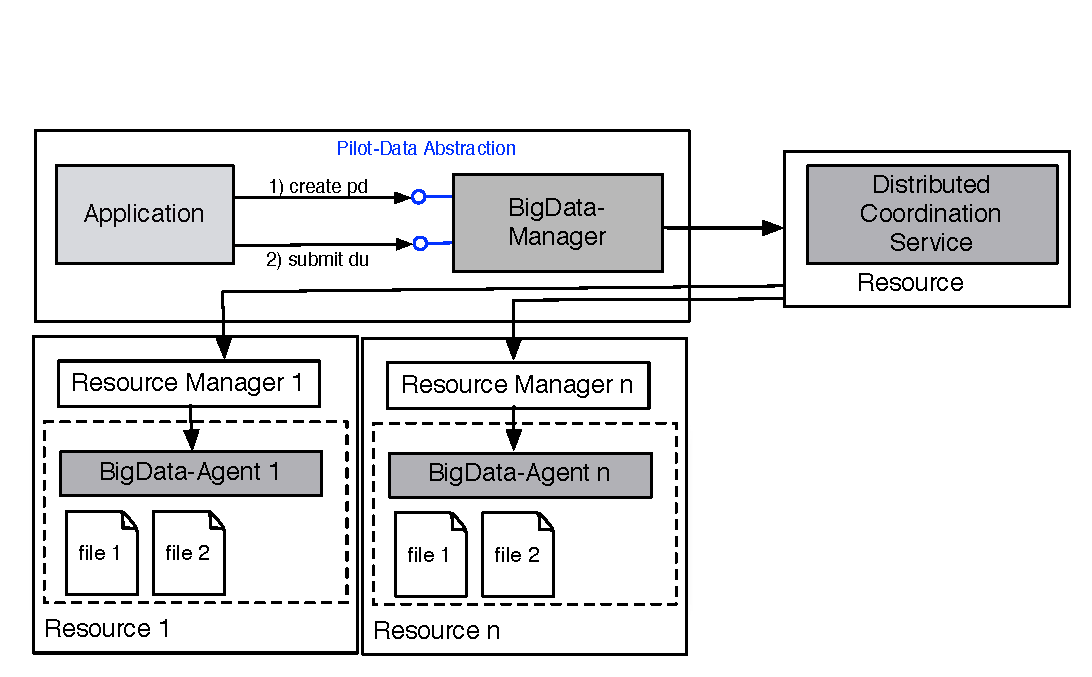
\includegraphics[width=0.48\textwidth]{../figures/bigdata_pmr.pdf}
	\caption{\I{\textbf{BigData Architecture and Interactions:}} Similar to BJ, a BD-Manager orchestrates a set of \pilots, i.\,e.\ BigData-Agent. Coordination is carried out via a distributed coordination service. \up\up }
	\label{fig:bigdata}
\end{figure}


BJ implements the following P* characteristic: As coordination model
the M/W scheme is used: The BJ-Manager is the central entity, which
manages the actual \pilot, the BJ-Agent. Each agent is responsible for
gathering local information, for pulling sub-jobs from the manager,
and for executing SUs on its local resource. The SAGA Advert Service
is used for communication between manager and agent. The Advert
Service (AS) exposes a shared data space that can be accessed by
manager and agent, which use the AS to realize a push/pull
communication pattern, i.\,e.\ the manager pushes a \su to the AS while
the agents periodically pull for new SUs. Results and state updates
are similarly pushed back from the agent to the manager. Further, BJ
provides a pluggable communication \& coordination layer and also
supports other \cc systems besides the AS, e.\,g.\ Redis~\cite{redis}
and ZeroMQ~\cite{zmq}.


%\subsection{BigData: A \pilotdata Implementation}

% Analogous to \pilotjobs, {\it Pilot-Data} (PD) abstraction provides late-binding
% capabilities for data by separating the storage allocation and application-level
% \dataunits~\cite{pstar-2012}. For this purpose, the API defines the {\it
% \pilotdata (PD)} and {\it \dataunit (DU)} entity: A \pd function as a
% placeholder object that reserves storage spaces for a set of \dus.
% 
% \begin{figure}[t]
% 	\upp\upp
% 	\centering
% 		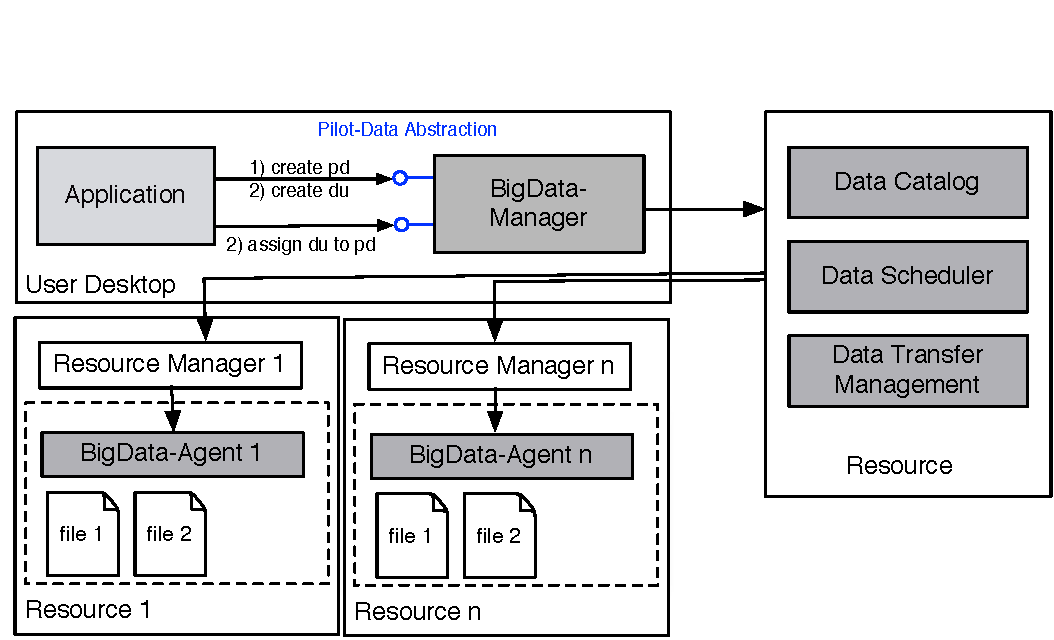
\includegraphics[width=0.4\textwidth]{figures/bigdata.pdf}
% 	\caption{BigData Architecture and Interactions\upp\upp\upp\upp\upp\upp}
% 	\label{fig:figures_bigdata}
% \end{figure}

{\it BigData (BD)} is an implementation of the Pilot-Data abstraction. BigData
is designed as an extension of BigJob. Figure~\ref{fig:bigdata}
provides an overview of the architecture of BigData. Similar to BigJob, it is
comprised of two components: the BD-Manager and the BD-Agents, which are
deployed on the physical resources. The coordination scheme used is
Master-Worker (MW), with some decentralized intelligence located at the
BD-Agent. The BD-Manager is responsible for (i) meta-data management, i.\,e.\
it keeps track of all \pd and associated \dus, (ii) for scheduling of data
movements and replications (taking into account the application requirements
defined via affinities), and (iii) for managing data movements activities.
BigData supports plug-able storage adaptors (currently for SSH,
WebHDFS~\cite{webhdfs} and Globus Online~\cite{10.1109/MIC.2011.64}).

% BJ currently uses a simple scheduling mechanism based on an internal queue: each
% \cu submitted to the BigJob framework is mapped to a \su. Binding can take place
% at submission time (early binding) or delayed in case of multiple \pilots (late
% binding). For scheduling, a simple FIFO queue is used (see also
% table~\ref{table:pilot-job-comparison}).


% In many scenarios it is beneficial to utilize multiple resources, e.\,g.\ to
% accelerate the time-to-completion or to provide resilience to resource failures
% and/or unexpected delays. BigJob allows dynamic resource additions/removals as
% well as late binding. The support of this feature depends on the backend used.
% To support this feature on top of various BigJob implementations that are by
% default restricted to single resource use, the concept of a BigJob pool is
% introduced. A BigJob pool consists of multiple BJs (each BigJob managing one
% particular resource). An extensible scheduler is used for dispatching \cus to
% one of the BJs of the pool (late binding). By default a FIFO scheduler is used.



% \note{OW says: Where is that magic BigJob-Pool and its scheduler? Is there an
% API for that? That's also part of the capabilities provided by
% bigjob-server.}\alnote{The BigJob pool is formerly known as ManyJob. In the
% bigjob/examples directory, there are multiple examples (e.g.
% example\_manyjob\_local.py) that show how multiple BJ can be used concurrently.}

% \input{sectionIV_comments}
\begin{table}[t]
\footnotesize
\centering
\begin{tabular}{p{2.4cm}p{1cm}p{1cm}p{1.95cm}p{2.0cm}}
  \toprule
  \textbf{P* Element}    &\textbf{BigJob} &\textbf{DIANE} &\textbf{Condor-G/ Glide-in}     \\\midrule
  Pilot-Manager          &BigJob Manager  & RunMaster     & condor\_master\newline 
                                                            condor\_collector\newline 
                                                            condor\_negotiator\newline 
                                                            condor\_schedd                        \\\midrule
  \pilot                 &BigJob Agent    & Worker Agent  &condor\_master\newline
                                                           condor\_startd                         \\\midrule
  \computeunit  \ (CU)   &Task            &Task           &Job                           \\\midrule
  Scheduling Unit (\su) &Sub-Job         &Task           &Job                           \\\bottomrule
% Dynamic Resources &no/yes &yes (AgentFactories)\\
% \hline
 \end{tabular}
 \caption{\I{\textbf{Mapping P* elements and PJ Frameworks:} While each PJ framework maintains its own vocabulary, each of the P* elements can be mapped to one (or more) components of the different PJ frameworks.
 }\up\up} 
 \label{table:bigjob-saga-diane}
\end{table}


% Binding 
% DIANE is primarily designed with respect to HTC environments (such as
% EGI~\cite{egi}), i.\,e.\ one PJ consists of a single worker agent with the
% size of 1 core.
% To use DIANE on HPC environments, a so-called multinode submitter script can be
% used: the scripts starts a defined number of worker agents on a certain
% resource.
% However, \cus will be constrained to the specific number of cores
% managed by a worker agent.
% By default a \cu  is mapped to a \su; application can however implement smarter
% allocation schemes, e.\,g.\ the clustering of multiple \cus into
% a \su.

%Scheduling


%Other impl. related issues: FT and security
% DIANE is, like BJ, a single-user PJ, i.\,e.\ each PJ is executed with the privileges
% of the respective user. Also, only \cus of this respective user are executed
% by DIANE. DIANE supports various middleware security mechanisms (e.\,g.\ GSI,
% X509). For this purpose it relies on GANGA.
% Further, DIANE supports fault tolerance: basic error detection and propagation
% mechanisms are in place. Further, an automatic re-execution of \cus is
% possible.






% \subsection{Swift/Coaster}
% 
% \jhanote{Eliminate?}
% 
% Swift~\cite{Wilde2011} is a scripting language designed for expressing
% abstract workflows and computations. The language provides, amongst many other
% things, capabilities for executing external applications, as well as the
% implicit management of data flows between application tasks. 
% % For this
% % purpose, Swift formalizes the way that applications can define
% % data-dependencies. Using so called mappers, these dependencies can be
% % easily extended to files or groups of files. 
% The runtime environment handles the allocation of resources and the spawning of 
% the compute tasks. 
% % Both data- and execution management capabilities are provided
% % via abstract interfaces. 
% Swift supports e.\,g.\ Globus, Condor and PBS resources. 
% % The pool of resources
% % that is used for an application is statically defined in a configuration file.
% % While this configuration file can refer to highly dynamic resources (such as OSG
% % resources), there is no possibility to manage this resource pool
% % programmatically. 
% By default, Swift uses a 1:1 mapping for \cus and \sus. However,
% Swift supports the grouping of SUs as well as PJs. For the PJ functionality, Swift uses the
% Coaster~\cite{coasters} framework. Coaster relies on a master/worker
% coordination model; communication is implemented using GSI-secured TCP sockets.
% Swift and Coaster support various scheduling mechanisms, e.\,g.\ a FIFO and a
% load-aware scheduler. Additionally, Swift can be used in conjunction with 
% Falkon~\cite{1362680}, which also provides \pilot-like functionality.

% Falkon
% refers to \pilots as the so called provisioner, which are created using the
% Globus GRAM service. The provisioner spawns a set of executor processes on the
% allocated resources, which are then responsible for managing the execution of
% SUs. \cus are submitted via a so called dispatcher service. Similar to Coaster,
% Falkon utilizes a M/W coordination model, i.\,e.\ the executors periodically
% query the dispatcher for new SUs. Web services are used for communication.

\subsection{Discussion}

P* provides an abstract model for describing and understanding PJ
frameworks, i.e., different components of PJ frameworks can be mapped
to the P* elements.  While each of the frameworks maintains its own
vocabulary, all share the common P* elements.
Table~\ref{table:bigjob-saga-diane} summarizes how P* can be applied
to BigJob, DIANE and Condor-G/Glide-in.
Table~\ref{table:pilot-job-comparison} summarizes the P*
characteristic and other properties of these frameworks. While most of
these frameworks share many properties, such as the M/W coordination
model, they differ in characteristics, such as communication model
or scheduling. \jhanote{OK, so the elements map to the different
  components, so what? what is the take home message?}


%Both BigJob and Swift have been
%developed for traditional US cyberinfrastructures, such as
%XSEDE. DIANE is native to EGI e-infrastructure.


% In the next section we will show how these frameworks can be exposed via the 
%Pilot-API.
% In addition to mapping the P* model to different PJ frameworks, we also
% expose BigJob, DIANE and Condor-G/Glide-in through the Pilot-API (see 
% section~\ref{sec:pilot-api}),
% i.\,e.\ the Pilot-API can now be used as a unified abstraction across
% multiple PJ frameworks (see figure~\ref{fig:figures_distributed_pilot_job}).  


\alnote{We haven't introduced the Pilot-API yet This validates (i)
the P* abstractions and (ii) the extensibility of the P*
model.}




% \note{TROY provides a
%   unified API that can be used to expose various PJ frameworks
%   (e.\,g.\ BigJob, DIANE and Condor-G). Further, it enables the
%   concurrent usage of multiple PJ frameworks (see
%   figure~\ref{fig:figures_distributed_pilot_job}). The SAGA inspired
%   approach to TROY's API design --- its SAGA inspired adaptor-based
%   architecture, leverage the design experiences of SAGA, are appealing
%   to the pilot-job user community. Also, the chosen designs enables
%   the easy exchange of PJ implementations and the concurrent use of
%   multiple PJ frameworks. TROY thus functions as common access layer
%   for different PJ frameworks, providing interoperability and
%   portability of PJ applications. To some extent, the TROY API can be
%   considered to be a prototype of a PJ-like API extension to SAGA (see
%   Discussion \& future work, \S\ref{sec:discussion-future-work}).}
% 


% \jhanote{It should probably be Coasters -- which is their notion of a
%   pilot-job.  Just to keep life interesting, they call it head-job and
%   not pilot-job!
%   \url{http://www.ci.uchicago.edu/swift/guides/release-0.92/userguide/coasters.php }}

% \alnote{Swift eval: no standard resource abstraction (SAGA),
%   proprietary language (not Python), TODO: check how coasters work!
%   1 coaster == 1 Condor-G job?}


%\subsubsection*{Other Pilot-Jobs and Conclusion}

% \jhanote{Can we add some structure to these *other* PJ.. this will be
%   ambitious and time-consuming, but if we can, that'll be (i) a great
%   service to the community, (ii) a strong intellectual addition to the
%   paper by virtue of validation of the P*-model}

% \alnote{which are the minimal P* elements and characteristics we
%   should discuss here?}  \jhanote{Andre L: Is this still a
%   valid/live comment/question? If not, should we close}\alnote{can
%   be closed.}

\begin{table}[t]
\footnotesize
\centering
\begin{tabular}{p{1.9cm}p{1.7cm}p{1.6cm}p{1.6cm}}
	\toprule
	\textbf{Properties}
	&\textbf{BigJob} &\textbf{DIANE} &\textbf{Condor-G/\newline Glide-in}    
	\\ \midrule

\textbf{Coordination} &M/W  &M/W &M/W \\ \midrule
	
\textbf{Communication} &Advert Service &CORBA &TCP\\ \midrule

% \midrule
% MPI/Multinode Applications &yes &no (yes with custom implementation of ApplicationWorker)\\
\textbf{Scheduling} &FIFO, custom &FIFO, custom &Matchmaking, priority-based scheduler \\

\I{Binding} & \I{Early/Late} & \I{Late} & \I{Late} \\


\midrule
Agent Submission &API &GANGA Submission Script &Condor CLI 
\\

\midrule

End User Environment &API &API and\newline M/W Framework  &CLI Tools \\ 

\midrule

Fault Tolerance &Error propa-\newline gation &Error propa-\newline gation, retries &Error propa-\newline gation, retries \\

\midrule

Resource Abstraction &SAGA &GANGA/\newline SAGA &Globus \\ 

\midrule

Security &Multiple\newline (GSI, User/Pass.) &Multiple (GSI) &Multiple\newline (GSI, 
Kerberos) \\ 

\bottomrule

% \hline
% Application Interfaces &Big-Job/Sub-job Management &Big-Job/Sub-job 
% Management\linebreak[4] Master/Worker API (\texttt{ITaskScheduler}, 
% \texttt{IApplicationManager}, \texttt{IApplicationWorker}) &&\\

	
\end{tabular}
\caption{\I{\textbf{P* Characteristics and Properties of Different Pilot-Job 
Frameworks:} The properties
in bold-face correspond to the P* characteristics; other items are general 
properties. The PJ frameworks share many P* characteristics and 
properties, e.\,g.\ the common usage of the M/W scheme or of a 
resource abstraction layer. However, they also differ in aspects, such as  
the coordination model or the communication framework. \upp
}\up\up}
\label{table:pilot-job-comparison}
\end{table}

%
%%%%%%%%%%%%%%%%% SECTION IV - Pilot-API %%%%%%%%%%%%%%%%%%%%%%%%%%%%
%

%\section{An API for the P*  Model\up}

\section{Pilot-API: A Uniform API to Heterogeneous PJ Frameworks}
\label{sec:pilot-api}


% \alnote{swap 3 and 4? Add mapping of API to PJ framework to API section}

% \terminology{TROY (implementation), P* Model, TROY API, PJ
%   implementation, BigJob, based on SAGA, PJ description, \cu 
%   description, TROY manager class, Condor Glide-in, DIANE, PJ-like
%   API extension) } \alnote{Lead: MS} \alnote{Renaming section and
%   subsections: TROY: A reference implementation of the P*}

In the previous two sections we presented successively the P* Model
and existing Pilot-Job frameworks. Before we present the Pilot-API --
which provides an abstract interface to Pilot-Job frameworks that
adhere to the P* Model, we will motivate the need for such an API.

\subsection{Motivation} 

\note{Reviewer Comment: In the end, the paper seems like a pilot job system
for pilot job systems. While the work seemed sound, I was unconvinced by the
paper that another layer of indirection and abstraction was the right solution
for connecting together pilot job systems. Perhaps another element which could
strengthen the paper is a description, based on the authors analysis of pilot
job systems, why pilot job systems cannot be unified in other ways.}

% 1) similar to workflows
% 2) system level vs. app level interop
% 3) leaky abstractions

% \jhanote{This section should cover threee points: (i) analogy to
%   workflow systems, (ii) different ways to interoperability -- API
%   (SAGA approach) is one, deeper semantic harmonization is the other,
%   (iii) in spite of limitation of API approach - leaky abstractions,
%   it is still useful, and in particular here..}


% Note to Shantenu:
%
%   There exist two ways toward system federation (i) deep integration
%   of systems (system level, interoperation), and (ii) abstract
%   interfaces (application level, integration).
%
% Shantenu, I do agree that the above version is possibly correct, and
% it gives me something to think about :-)  But for the purpose of the
% paper, it may actually complicate things.  For one, our discussion
% of WFs below does not distinguish between interoperation and
% integration, and adding that distinction is adding noise to the text
% (I tried that, it reads aweful).
% 
% More importantly, we user interoperation elsewhere in the text, for
% example when we talk about "Understanding PJ Framework
% Interoperability".  Now, on that level we do not really do interop,
% according to the definition above, but integration (we change none
% of the systems internally, apart from possibly bigjob).  So, we
% would have to change that discussion to integration, which is, while
% being correct I think, complicating the discussion, and also
% somewhat less intuitive for the reader (I think).
% 
% I thus left the definition for now, but please feel free to change
% it, if you feel that the increased correctnes is worth the effort to
% keep the paper consistent.

At a high-level, there exist two approaches towards interoperability:
(i) deep integration of systems (system level interoperability), and
(ii) the use abstract interfaces (application level interoperability).
Approach (i) requires a certain level of semantic harmonization
between the systems, and is (in principle and technically) hard to
achieve post-facto, even if the respective systems inherently
implement the same abstract model (here: the P* Model).  While
interoperation via an abstract interface (ii) (here: Pilot-API) is a
semantically weaker approach than (i), it does allow for
interoperability with minimal (application level)
effort~\cite{saga_bigjob_condor_cloud,saga_gin}.


% Workflow (WF) capabilities and engines are typically tied to specific
% tools and infrastructure (e.\,g.\ DAGMan-Condor) and require the
% adaption of the application to the WF engine as opposed to the other
% way around. 

The current state of workflow (WF) systems~\cite{nsf-workflow,1196459}
provides a motivating example for the P* Model and the Pilot-API:
even though many WF systems exist (with significant duplicated
effort), they provide limited means for extensibility and
interoperability.  We are not naive enough to suggest a single reason,
but assert that one important contributing fact is the lack of the
right interface abstractions upon which to construct workflow systems;
had those been available, many/most WF engines would have likely
utilized them (or parts thereof), instead of introducing proprietary solutions.
%
% That would not immediately allow WF implementations to interoperate,
% but would make semantic mapping between them significantly simpler,
% thus supporting the very notion of interoperation.
%
Significant effort has been invested towards WF interoperability at
different levels -- if nothing else, providing post-facto
justification of its importance. The impact of missing interface
abstractions on the WF world can be seen through the consequences of
their absence: WF interoperability remains difficult if not
infeasible. The Pilot-API in conjunction with the P* Model aims to
prevent similar situation for \pilotjobs.

%\footnote{To be fair: we are not sure if a generic model and/or a
%  generic WF API are achievable {\it on a useful level} -- we think,
%  nevertherless, that our discussion is valid.}


% \jhanote{Somewhere we need to define the different approaches to
%   interoperability. One is via the interface/API; the other is via
%   deeper integration. In the former the lowest common denominator
%   approach is employed. In the latter semantic differences are
%   addressed but at different levels} \alnote{elaborate on
%   SAGA-based approach to interoperability: We use the the API approach
%   to interoperability => talk about approach not api}\jhanote{ditto}
% 
% \note{1) provide expose model 2) api-level interoperability}

% \jhanote{Please elaborate the following} It is also consistent with
% SAGA in that it can support the same underlying job-model...
% \jhanote{ not sure about the relevance of the following sentence:}

We appreciate the difficulty balancing the level of semantic
expressivity for API's designed to work on multiple semantically
heterogeneous systems: defining the API as 'smallest common
denominator' is often too simplifying and misses large numbers of
'edge' use cases; defining the API as 'greatest common factor'
clutters the API with non-portable semantics, making the API too
complex~\cite{leaky_abstractions}.  The Pilot-API uses the Pareto
principle as guideline for a balanced abstraction level.

\begin{figure}[h]
    \begin{center}
    \up
    \includegraphics[width=0.47\textwidth]{../figures/distributed_pilot_job.pdf}
    \caption{\I{\textbf{Pilot-API and PJ frameworks:} The Pilot-API provides 
      a unified interface to utilize the native Pilot-Job capabilities of
      different infrastructures, e.\,g.\ BigJob for XSEDE/FutureGrid
      resources, DIANE for EGI and Condor for OSG resources.
      % It also enables the concurrent usage of these infrastructures.
  \up\up
  }\label{fig:figures_distributed_pilot_job}}
  \end{center}
\note{Reviewer Comment: The experiments are by far the weakest part of this paper. For the experiments parts, the authors didn't explain very well how they test the interoperability between Pilot-Jobs and infrastructures exist. The results are also hard to follow, why certain experiments are done, and how to interpret the results.}
    
\end{figure}


% While no single solution can address
% all levels nor the entire spectrum of applications, the Pilot-API
% exposes effective abstractions that can hide environmental complexity,
% supplement the incompleteness and lack-of-extensibility of many tools,
% and generalize customized run-time solutions for a broad range of
% applications. 


% \amnote{according to Shantenu, 'abstraction' is over-used in the text
% above.  I changed some occurences, but more remain which I am not sure
% how to replace without increasing noise.}

% MS: commented out the next session as it talks about the runtime system
% The pilot-job capabilities in TROY are provided by different PJ
% frameworks that are integrated into the TROY runtime system via
% adaptors. For this purpose, TROY defines a Capability Provider
% Interface (CPI) that must be implemented by the adaptors of the
% underlying pilot-job frameworks. This architecture also enables the
% concurrent usage of multiple PJ frameworks.  \jhanote{NO mention of
%  CPI should occur}

% \begin{figure}[t]
% 	\upp
% 	\centering
% 		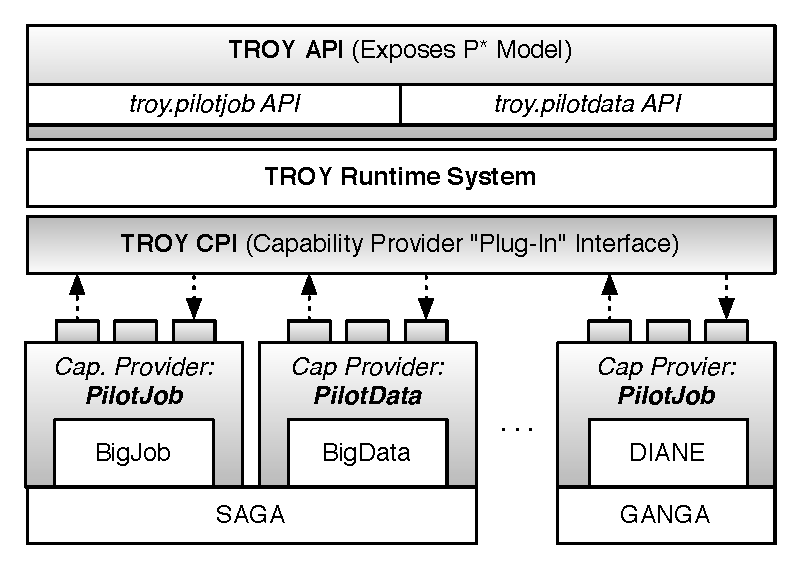
\includegraphics[width=0.45\textwidth]{figures/TROY_arch.pdf}
%                 \caption{\I{\textbf{TROY -- An API and Runtime System for
%                     the P* Model:} TROY provides an API for managing
%                   PJs and PDs. BigJob and BigData are realizations of
%                   the actual PJ and PD functionality. BJ and BD rely
%                   on SAGA for implementation of the PJ/PD.}}
% 	\label{fig:figures_pstar_troy}
% 	\up
% \end{figure}


\subsection{Understanding the Pilot-API}

% \alnote{We don't establish that the BJ API is semantically equivalent to the 
% Pilot-API.}

The Pilot-API~\cite{pilot_api} is a Python-based API and supports two different usage modes (i)
it provides a unified API to various PJ frameworks (e.\,g.\ BigJob, DIANE and
Condor-G/Glide-in), and (ii) it enables the concurrent usage of multiple PJ
frameworks.

The Pilot-API classes and interactions are designed to reflect the P*
elements and characteristics.
% Table~\ref{table:pstar_elements} summarizes the mapping of P* elements and the
% Pilot-API.
The API exposes the primary functionality of the Pilot-Manager using two
classes: the \texttt{Pilot\-Compute\-Service} for the management of \pilots
and the \texttt{Compute\-Unit\-Service} for the management of \cus. 
As defined by P*, a \cu represents a primary self-containing piece of work that
is submitted through the Pilot-API. 
%At the API boundary a \cu transitions to a \su, which functions as internal unit
%of scheduling.

Figure~\ref{fig:figures_pilot_api_flow} shows the interactions between the
Pilot-API entities. The Pilot-API decouples
workload management and resource scheduling by exposing two separate services: 
The \texttt{Pilot\-Compute\-Service} and
\texttt{Compute\-Unit\-Service}. 
The \texttt{Pilot\-Compute\-Service} serves as a factory for instantiating \pilots. 
Also, the \texttt{Pilot\-Compute\-Service} can be used to query for currently
active \texttt{Pilot\-Compute} instan\-ces.
A \texttt{Pilot\-Compute} instance is returned as result of the
\texttt{create\_pilot()} method of the \texttt{Pi\-lot\-Compute\-Service} (step 1).
The instantiation of the
\texttt{Pilot\-Compute} instance is done by using a
\texttt{Pilot\-ComputeDescription}. The description can be reused and has no
state, while the \texttt{Pilot\-Compute} instance has state and is a reference
for further usage:
the references \texttt{Pilot\-Compute} object represents a \pilot instance and allows the 
application to interact with it, e.\,g.\ to query its state or to cancel 
it. The process of \texttt{Pilot\-Compute} creation is depicted in step 1-2 of 
figure~\ref{fig:figures_pilot_api_flow} and in listing~\ref{lst:pcs_creation}.\\


\lstset{
language=Python,
frame=single,
captionpos=b,
stringstyle=\ttfamily,
basicstyle=\scriptsize\ttfamily
}

\begin{minipage}{0.45 \textwidth}
\begin{lstlisting}[caption={\I{Creation of a \T{PilotCompute} instance using a \T{Pi\-lot\-Compute\-Description}.}}, label={lst:pcs_creation}]
pcs = PilotComputeService()
pc_desc = PilotComputeDescription()
pc_desc.total_core_count = 8
pc = pcs.create_pilot('gram://queenbee', 
                          pc_desc, 'bigjob')
\end{lstlisting}
\end{minipage}

Listing~\ref{lst:cus_creation} shows the creation of
a \texttt{Compute\-Unit\-Service}.  Having created
a \texttt{Compute\-Unit\-Service} instance, \texttt{Pilot\-Compute\-Service}
instances can be added and removed at any time, which makes the respective pilots available to that Service.  These semantics enable applications to
respond to dynamic resource requirements at runtime, i.\,e.\ additional
resources can be requested on peak demands, and can be released if they are no
longer required.\\

\begin{minipage}{0.45 \textwidth}
\begin{lstlisting}[caption={\I{Instantiation
of a \texttt{ComputeUnitService} using a reference to the
\texttt{PilotComputeService}.}}, label={lst:cus_creation}]
cus = ComputeUnitService()
cus.add(pcs)
\end{lstlisting}
\end{minipage}

% \lstset{
% caption={\textbf{WorkUnit Submission:} Instantiation and Submission of a \texttt{WorkUnitDescription}.\label{lst:submission}}
% }

The \texttt{Compute\-Unit\-Service} is responsible for managing the execution of
\cus.
Regardless of the state of the \texttt{Pilot\-Compute\-Service}, applications can submit \cus to a
\texttt{Compute\-Unit\-Service} at anytime (listing~\ref{lst:submission} and step 3
in figure~\ref{fig:figures_pilot_api_flow}). 
Once the \texttt{Compute\-Unit\-Service} becomes responsible for a \cu, the \cu
transitions to an \su.
SUs are internally processed (e.\,g.\ they can be aggregated) and are then scheduled to the Pilot-Job Framework (step 4). 
The PJ framework is responsible for the actual execution of the \su on a
resource.
Note that multiple levels of (hierarchical) scheduling can be present -- commonly
a \su is scheduled inside a PJ framework, the model allows it to be present
in multiple layers.\\

\begin{minipage}{0.45 \textwidth}
\begin{lstlisting}[caption={\I{Instantiation and 
	submission of a \texttt{Compute\-Unit\-Description}.}}, label={lst:submission}] 
cud = ComputeUnitDescription()
cud.executable = '/bin/bfast'
cud.arguments = ['match', '-t4', '/data/file1']
cud.total_core_count = 4
cu = cus.submit(cud)
\end{lstlisting}
\end{minipage}



% In figure~\ref{fig:figures_pilot_api_flow} the flow of a simple execution scenario is
% displayed. The Pilot Job Service and the Work Unit Service are already
% instantiated. The application requests the Pilot Job Service to create a new
% pilot-job (step 1), the Pilot Job Service will pass the request on to the
% relevant adaptor (step 2), which will eventually launch the pilot-job on a
% resource using a pilot-job framework (step 3). At this stage there might be a
% pilot-job already available, or the request can still reside in a queue
% somewhere. Regardless of the state of the pilot-job, the application can submit
% a work unit to the Work Unit Service (step 4). The Work Unit Service remains
% responsible for keeping track of the Work Unit during its lifetime. Based on the
% heuristics or policies the WUS decides on a potential aggregation of
% SUs. The \su 
% is then forwarded to the Scheduler (step 5). The Scheduler will schedule SUs to 
% an appropriate adaptor that represents a capable resource (step 6). Finally, the
% adaptor will submit the \su to the PJ framework which will
% take care of the actual execution on a resource. Note that multiple levels of 
% (hierarchical) scheduling can be present. Inside
% TROY there is already scheduling taking place inside the Work Unit Service. 
% Additionally, the underlying PJ framework can conduct its own scheduling.


Each \texttt{Compute\-Unit} and \texttt{Pilot\-Compute} object is associated
with a state.
The state model is well defined --
% based on the SAGA job state model~\cite{ogf-gfd-90}.
applications can query the state using the \texttt{get\_state()} method or they
can subscribe to state update notifications (by setting callbacks).

Finally, an application can have any number of \texttt{Pilot\-Compute\-Service} or
\texttt{Compute\-Unit\-Service} instances.
Multiple \texttt{Pilot\-Compute\-Service} instances can be associated to a
\texttt{Compute\-Unit\-Service}, and a \texttt{Pilot\-Compute\-Service} can be associated to
multiple \texttt{Compute\-Unit\-Service} instances.
A \texttt{Compute\-Unit\-Service} can manage multiple \texttt{Compute\-Unit}
instances, but a \texttt{Compute\-Unit} can only be managed by one
\texttt{Compute\-Unit\-Service}.
Similarly, a \texttt{Pilot\-Compute\-Service} can manage multiple
\texttt{Pilot\-Compute} instances, but a \texttt{Pilot\-Compute} can only be
managed by one \texttt{Pilot\-Compute\-Service}.


\begin{figure}[t]
	\centering
  \upp\up
		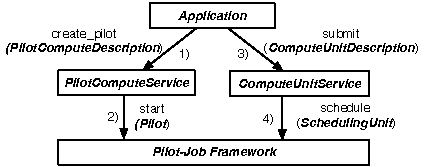
\includegraphics[width=0.48\textwidth]{../figures/pilot-api-flow.pdf}
	\caption{\I{\textbf{Control Flow Pilot-API and PJ Frameworks:} The 
	functionality of pilot-jobs are exposed using two primary classes: The 
	\texttt{Pilot\-Compute\-Service} for the management 
	of \pilots, and the \texttt{Compute\-Unit\-Service} for the management of 
	\cus. \up\up
	}}
	\label{fig:figures_pilot_api_flow}
\end{figure}

%\begin{table}[t]
%	\centering
%\begin{tabular}{|l|l|}
%\hline
%\textbf{Pilot} &PJ framework\\
%\hline
%\textbf{\cu } &\cu \\
%\hline
%\textbf{\su} &\su\\
%\hline
%\textbf{Pilot-Manager} & PilotComputeService/ComputeUnitService\\
%\hline
%\end{tabular}
%\caption{Mapping of P* and the Pilot-API\up
%\msnote{\\\\I find this a rather unuseful table and can be axed if you ask me}
%}\label{table:pstar_elements}
%\end{table}


\subsection{Pilot-API for Data}

Analogous to the Pilot-API for Compute, the Pilot Data
API~\cite{pilot_api} defines the \texttt{PilotDataService} entity as
an abstraction for creating and managing pools of storage. A
\texttt{PilotData} instance represents the actual physical storage
space. An additional \texttt{ComputeDataService} entity functions as an
application-level scheduler, which accepts both
\texttt{Compute\-Units} and \texttt{DataUnits} -- this resolves new
dependencies (e.g. data/data or data/computer affinities), and is
responsible for managing the execution of \dus and \cus.

\section{Experiments and Results}\label{sec:exp_res}

\note{Reviewer Note: Unfortunately, the experimental results are not
  very convincing. Firstly, the overhead caused by interoperability
  (P*) is not provided. And the introduced overheads are critical in
  understanding if it is a worthwhile approach. Secondly, the
  demonstration of interoperability is overly simplified. For example,
  so of these pilot job systems were never meant to operate decoupled
  from their computational frameworks. For example, Swift and
  Swift-Coasters were meant to work together. It’s not clear how one
  would interact with Swift-Coasters, without generating Swiftscript
  code (as opposed to simple job/task descriptions). The Swiftscript
  is very much a special instance of a way to implement some
  application logic. I would find it hard to believe that an
  application could adapt to such different requirements, where some
  application could be converted between some collection of jobs, to a
  Dagman/Condor workflow, to a Swift-Coaster workflow, and all this to
  be done automatically. If the complex workflow dependency management
  is taken out of the equation, then why bother to talk about the
  features of these workflow systems, such as the data from Table 2?
  More metrics like traffic, slowdown, and job speedup are needed to
  be measured to be convincing.}

\note{Reviewer Comment: The experiments are by far the weakest part of
  this paper. For the experiments parts, the authors didn't explain
  very well how they test the interoperability between Pilot-Jobs and
  infrastructures exist.  The results are also hard to follow, why
  certain experiments are done, and how to interpret the
  results. Experiments are not clear enough to support the
  arguments. Does not say how to handle the case if the function in
  the framework can not be map to the P* Model. Also, I was expecting
  that more time would be spend on the Pilot-Data model, and how this
  translated to the various pilot-based systems.}

% In this section we analyze the performance and scalability of
% different PJ frameworks. 

As discussed in \S\ref{sec:pilot-job-frameworks}, several PJ frameworks can be
collectively used via the Pilot-API.  We begin by understanding the overhead of
PJ frameworks (section~\ref{sec:pj_performance}).  In
section~\ref{sec:fg-xsede-osg-egi} we show the effectiveness of the

Pilot-API/P* Model approach by executing {\it real application
workloads} -- a genome alignment application -- on multiple distinct
production infrastructures. It is important to note that our
experiments do not try to identify the ``fastest'' PJ framework, as
this is dependent on different factors, e.\,g.\ particularly the
infrastructure used.  Experiments are conducted on different
production (XSEDE, EGI, OSG) and research (FutureGrid)
infrastructures.  Further, we demonstrate interoperability by using
multiple PJ frameworks concurrently on multiple infrastructures using
the Pilot-API -- see section~\ref{sec:experiment-interop}.  

\jhanote{We should agree on what the
last set of experiments are trying to convey/achieve}


% of performance and scalability of coordination in BigJob and DIANE,
% executing thousands of tasks but with zero workload. We establish that
% for up to thousands of tasks, existing coordination infrastructures
% suffice. \jhanote{We don't do the previous two sentences, do we?}
% \alnote{Well we did, but the figure is now not part of the paper
%   anymore. We could say hundreds of concurrent tasks}


% \jhanote{Need a simple description of experiment   configuration}.
% \alnote{Is it ok to just describe the configuration on high-level in the 
% introduction and do this in detail in the sub-sections?}\jhanote{yes}

% \alnote{this paragraph is redundant to B and C? Alternative we can move
% stuff from there to here.}
% For purposes of validation, demonstration and performance
% measurements, we use the Pilot-API to marshall different PJ
% frameworks...  The experiments are conducted on different
% production (XSEDE, EGI, OSG) and research infrastructures
% (FutureGrid).

% \jhanote{Need to provide details of the application} 
% \alnote{Is it ok to do this in subsection B and C?}\jhanote{yes} 

%(with SAGA/PBS and SAGA/Condor) and DIANE in a genome sequencing
%application scenario.



% \amnote{Someone please check the above statement for sanity!}
% \alnote{What's a concertation?}  \amnote{wiktionary says: "A form of
%   dialogue and co-decision, implying the mutual exchange of
%   information, open discussion and knowledge sharing, and the
%   signature of operational agreements between public administrations
%   and/or with representatives of the private sector."  Basically
%   means in our context 'in a coordinated way, in
%   combination'.}\jhanote{Would `` collectively'' be a better
%   description?}

\subsection{PJ Frameworks Overheads}\label{sec:pj_performance}

% \alnote{What are the factors for overheads? coordination, file
%   staging, file systems, job submission? invoke SAGA Europar?}
% \jhanote{We should explicitly mention the Pilot-API overhead, even if
%   only to state that it is effectively zero! Don't leave anything
%   to the imaginatino of the reviewer!} \alnote{refined}

% Different PJ implementation follow different design objectives --
% that also reflects in the designs of their communication \& coordination 
% (\cc) sub-systems. 
%(see~\cite{denBurger:2010:PSC:1887695.1887739} 

Before we understand the performance of different frameworks for real
application workloads, we analyze the typical overheads for BigJob and DIANE.
The overhead of a PJ framework, like many
distributed submission mechanisms and tools, is most commonly determined by
the following factors: the API overhead, the job submission and coordination
overhead. Although important determinants of the time-to-solution, the
queueing and file staging time heavily depend on extrinsic factors, such as
the system and network load, but are not intrinsic overheads of the PJ
framework. The overhead of the API-layer, i.\,e.\ the Pilot-API, was not 
measurable using the built-in Python profiler, which provides accuracies in 
the magnitude of milliseconds. Also, we previously established that job 
submission times are commonly very low compared in particular when compared to 
the overall runtime~\cite{saga_europar10}.  Thus, we focus our investigation on the distributed coordination overhead. There are many factors
that influence the overall coordination performance, e.\,g.\ the
degree of distribution (local (LAN) vs. remote (WAN)), the
communication pattern (1:n versus n:n) and the communication
frequency.
% Thus, the primary barrier for performance and scalability is not the
% internal coordination of the elements of a PJ implementation. 




 
% To evaluate \cc overheads, we conducted several experiments on
% FutureGrid~\cite{fg}. 



% In the following we investigate the impact of different \cc related
% factors on the overall performance and scalability of PJ systems.
% We evaluate different BigJob configurations, and compare and
% contrast them with DIANE.

% BigJob's \cc was originally based on a shared, centralized data space, 
% the SAGA Advert Service (AS)~\cite{saga_advert}.  The
% communication between all components is done via this shared data
% space, which decouples BJ-Manager and BJ-Agent and allows both
% entities to operate at their own pace, optimizing the overall
% throughput.  A particular 

% An issue during distributed runs is the latency
% between the application and the (remote) Advert Service. Another
% challenge is that this design introduces a potential
% single-point-of-failure and scalability bottleneck if the centralized
% data space is not carefully designed and operated.

% BigJob also provides two alternative c\&c sub-systems:
% Redis~\cite{redis} and ZeroMQ~\cite{zmq}. Redis is a lightweight
% key/value store. Redis is used in a similar way as the AS, i.\,e.\ all 
% communication between BJ-Agent and BJ-Manager is
% channeled through it. In contrast, the ZeroMQ sub-system utilizes a
% client-server architecture, which is similar to the CORBA-based approach 
% of DIANE -- in this architecture, the PM maintains the
% overall state. Clients connect to the PM to request new SUs or to
% report state updates. An advantage of this architecture is that it
% does not require a separate infrastructure deployment for the \cc
% sub-system.

% Both the data space and the client-server \cc sub-systems can be
% combined with a publish/subscribe mechanism, i.\,e.\ instead of
% polling, an agent can receive notifications when a new \su arrives.

% \jhanote{Need to motivate testing of c\&c sub-system better: There
%   are many barriers to interoperability and performance. Primary
%   barrier to performance is not \cu submission or \su scheduling to
%   PM, but the fundamental limitation of scalability of coordination
%   -- with increasing number of \cu /\su.  Establish tradeoff between
%   distributed vs local coordination. e.g., It is easy to get
%   consistency but has overhead.  Easy to get performance but
%   difficult to get consistency. Thus we opt for centralized /
%   persistent point. But how does this single point-of-coordination
%   behave with increasing number of connections? } \alnote{hopefully
%   addressed most points in paragraph above}

% \begin{figure*}[htbp]
% 	\centering		
% 	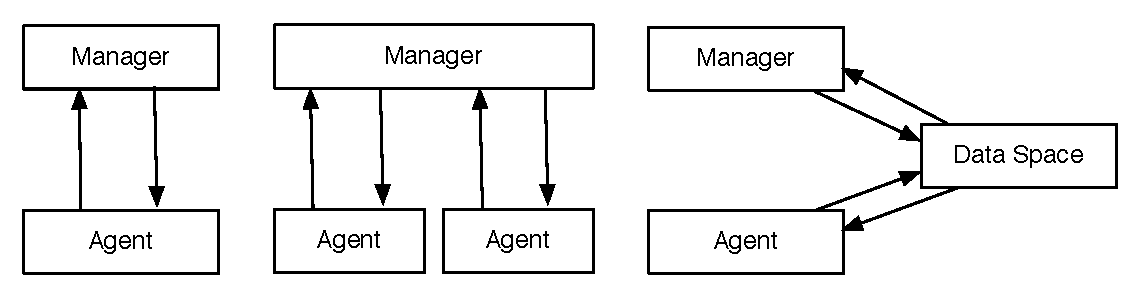
\includegraphics[width=0.8\textwidth]{figures/coordination-schemes.pdf}
% 	\caption{\textbf{Coordination \& Communication:} The primarily
%    used coordination pattern is the utilization of a
%    request/response server (left, middle). In the data-space model
%    (right) all application components are connect to a central
%    data-space. This architecture decouples manager and agent
%    allowing both to operate on its own pace.}
% 	\label{fig:figures_coordination-schemes}
% \end{figure*}

% Figure~\ref{fig:figures_coordination-schemes} illustrates different
% coordination schemes. 

% Most pilot-jobs utilize the master-worker \jhanote{M-W for what?}
% pattern commonly implemented on basis of a simple request/response
% architecture, i.\,e.\ the \jwave{agent} sends a request for work
% packages to the master, which replies with a \cu . 

% \jhanote{Are we talking specific implementation, i.e., TROY? If so we
%   should not say ``A'' manager but ``The Pilot-Manager''? Also the previous
% sentence should not talk about most pilot-jobs, if we've already started
% talking about TROY!!} \alnote{hopefully fixed.} 

% A manager
% can manage a single agent (e.\,g.\ BigJob) or multiple agents
% (e.\,g.\ DIANE). 


% \begin{figure}[htbp] 
%  \centering
%  %\up
%  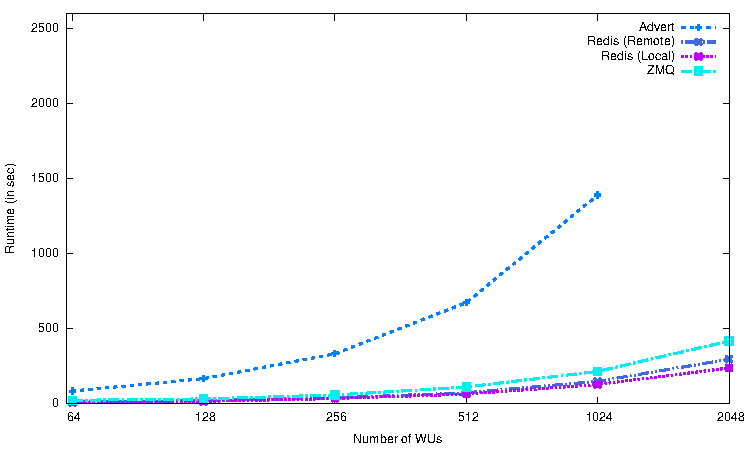
\includegraphics[width=0.49\textwidth]{../perf/bigjob-varying-wus-alamo.pdf}
%  \up\up
%  \caption{\textbf{BigJob and DIANE Performance (1):} The 
%   runtime increases linearly with the number of \cus in most cases. 
%   The overhead per \cu imposed by the AS is generally 
%   higher than for other backends. The runtime of the DIANE \cus only increases 
%   moderately mainly due to the aggregation of the \cus.
%   %\up
% }
%  \label{fig:perf_bigjob-varying-wus} 
% \end{figure}
% 
% Figure~\ref{fig:perf_bigjob-varying-wus} illustrates the performance
% and scalability of different BJ configurations and DIANE with
% respect to the number of \cus. Clearly, the \cc sub-system has a great
% impact on the overall performance: the Redis backend shows the best
% performance for small \cu counts. The difference between local and
% remote coordination is moderate (about 20\,\%). While ZeroMQ is very
% fast and lightweight, it requires a careful implementation, in
% particular concerning synchronization and throughput optimization. The
% overall performance is slightly worse than for Redis. The Advert
% Service currently has some limitations which will be discussed later.
% DIANE shows a higher startup overhead, which is particularly
% observable for smaller \cu  numbers. However, the runtime increases only 
% slightly (about 10\,sec) when going from 64 to 2048 \cus. One reason is that 
% DIANE aggregates SUs: for 2048 \cus only a single task description is created, 
% which the framework efficiently distributes to its agents. BigJob in contrast 
% maintains a separate description for each \cu.
% At the investigated scales, the single manager does not represent a
% bottleneck with respect to the processable \cu  numbers. Further,
% the TROY manager introduces another hierarchy-level which can
% further enhance the overall scalability.

% As in the last experiment,
% the Advert \cc sub-system showed a significantly lower performance.
% A reason for that
% is the used remote access protocol, which is basically the native
% remote PostgreSQL database protocol, which is not optimized for WAN
% connections. Further, the API is based on a hierarchical namespace,
% which does not easily map to relational databases -- in deeply nested
% namespaces exhibit an insufficient query and update performance. In
% contrast, data is stored in memory for Redis and ZeroMQ, which
% explains the significant performance gains.

% \jhanote{at times i think this whole subsection can be removed and
%   replaced by a paragraph that summarises (i) the architecture (ii)
%   the challenge (iii) performance measurement and analysis?}


% One reason is that 
% DIANE aggregates SUs: for 2048 \cus only a single task description is created, 
% which the framework efficiently distributes to its agents. BigJob in contrast 
% maintains a separate description for each \cu.
% At the investigated scales, the single manager does not represent a
% bottleneck with respect to the processable \cu  numbers. Further,
% the TROY manager introduces another hierarchy-level which can
% further enhance the overall scalability.

% \jhanote{Need to mention this is for BigJob and not PJ frameworks in
%   general, as it reads now!}\alnote{ok}

We executed a different number of very short running (i.\,e. zero workload)
\cus on Alamo/FG concurrently. 
% \pmnote{what figure does it refer
% to..Not sure what experiments done on Alamo?} \alnote{yes, this was on Alamo}
This enables us to focus on the overhead induced by the \cc subsystem. Each
experiment is repeated at least 10 times. In general, the c\&c systems used
are mostly insensitive to the number of coordinated \cus.
%\onote{Strong claim -- data doesn't show any significant scale-up} 
Although we do not provide a detailed discussion of the dependency between 
coordination overhead and the number of \cus, it is worth mentioning that the 
runtime increases only slightly with the size of the pilot and/or the number of managed \cus.

\jhanote{Is this c\&c overhead?} \pmnote{what machines are used to run BigJob, 
are all these compute units executed concurrently using BigJob and Diane?} 
Figure~\ref{fig:perf_bigjob-varying-cores} illustrates the performance
scalability with respect to the number of cores and \cus managed by \pilot. 
For this purpose,
we execute 4\,\cus per core, i.\,e.\ between 32 and 512\,\cus. BigJob with
Redis (local) shows almost linear scaling up to 128 cores. BigJob with Redis
(remote) imposes an overhead of about 14\,\%. BigJob with ZeroMQ performs very
well with lower core counts; with larger core counts, the runtimes increase,
indicating a potential scalability bottleneck. DIANE shows, in particular for
lower core counts, a longer runtime, again due to higher startup overhead.
With higher core counts DIANE behaves similar to BigJob/ZeroMQ, but shows a
greater increase of the overall runtime. This increase is likely attributable
to the single central manager in DIANE's CORBA-based client-server
architecture. Using Redis as central data space for BigJob decouples 
Pilot-Manager and Agent, yielding better performance in
particular with many replicas.

\begin{figure}[t] \centering \up\up
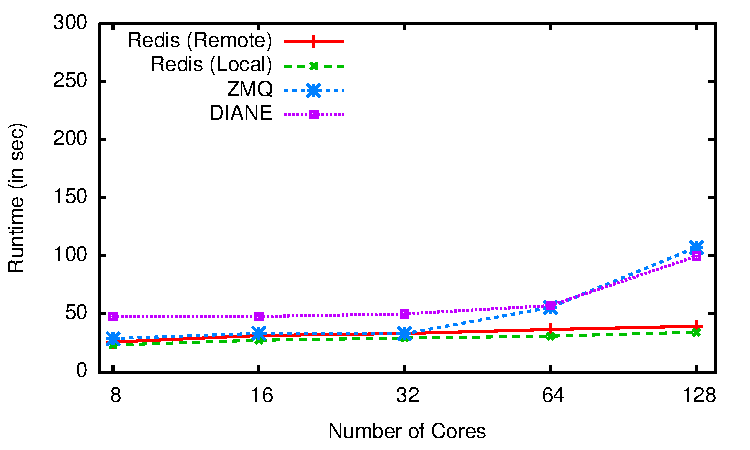
\includegraphics[width=0.4\textwidth]{../perf/bigjob-varying-cores-alamo-noadvert.pdf}
\upp \caption{\I{\textbf{\pilotjob Coordination Mechanism:}  The runtime of a
workload of 4 \cus per core, i.\,e.\ 32 - 512\,\cus, using different \pilots
and configuration. For BJ-Redis the runtime  increases only moderately, the
client-server-based implementations BJ-ZMQ and CORBA-based DIANE show
particularly a steep increase when going from 64 to 128 cores. \up\up }}
\label{fig:perf_bigjob-varying-cores} \end{figure}

% The AS implementation currently shows some performance
% limitations, mainly caused by the prototypical nature of its
% implementation.  Further, it must be noted that the Advert Service was
% deployed remotely (mainly due to deployment constraints). Even so, the
% discrepancy between AS and Redis (Remote), which has been
% deployed on the same remote network, is significant. A reason for that
% is the used remote access protocol, which is basically the native
% remote PostgreSQL database protocol, which is not optimized for WAN
% connections.
%
% \jhanote{It is not clear why REDIS and ZeroMQ are not susceptible to
% access over WAN delays/latency?}\alnote{included a comparison note
% to Redis Remote. We can't compare it to ZMQ since we use only local
% communication in this case}
%
% Transactions e.\,g.\ are very latency sensitive and require several
% roundtrips.  Further, the API is based on a hierarchical namespace,
% which does not easily map to relational databases -- in deeply nested
% namespaces exhibit an insufficient query and update performance. In
% contrast, data is stored in memory for Redis and ZeroMQ, which
% partially explains the significant performance gains.

\subsection{Characterizing PJ Frameworks on DCI}
\label{sec:fg-xsede-osg-egi}


%\subsubsection*{Production Infrastructure} 

To validate the effectiveness and usability of the Pilot-API, we
conducted a series of experiments on various production infrastructures. We
executed BFAST~\cite{bfast2009} using three different PJ frameworks (BigJob,
DIANE and Condor) on XSEDE~\cite{xsede}, FutureGrid~\cite{fg}, EGI~\cite{egi}
and OSG~\cite{1742-6596-78-1-012057}.

Specifically, we utilized the following resources: XSEDE: Trestles 
(100\,TFlop / 324\,nodes / 10,368\,cores / Torque) and QueenBee
(Linux Cluster / 668\,nodes / 5,344\,cores / PBS); FutureGrid:
India and Sierra (108\,nodes / 864\,cores / PBS); 
%\pmnote{sierra needs to be included}\alnote{ok} 
European Grid Initiative (EGI): Resource federation of 364,500 cores;
OSG: Condor pool (via the \textit{Engage} VO, GlideinWMS,
20,000 Glide-ins).\footnote{GlideinWMS is a software system built on
top of Condor-G/Glide-in, which can, based on the current and expected
number of jobs in the pool,  automatically increase or decrease the
number of active Glide-ins (\pilots) available to the pool.  While the
average number of active Glide-ins on OSG is around 20,000, more than
40,000 Glide-ins can be active and available for job execution during
peak load.}

 
%\jhanote{I would even introduce a sub-subsection on production
%  infrastructure used. That would enable us to keep Pilot-API/BigJob
%  specific details separate from infrastructure details. E.g., say
%  what is XSEDE? Say what is OSG? Thoughts?}  \alnote{good
%  idea. started to restructure section}


%\note{OW says: That would be the case if we use Condor-G. The machines
%is belhaven-1.renci.org - a Globus/PBS cluster that accepts Condor jobs.\\
%So the OSG is a peculiar beast. My current understanding is, that it consits 
%of a bunch of HPC clusters with a Globus frontend. OSG uses an automated 
%Glide-in WMS service that starts glide-ins via Condor-G on these clusters.
%The glide-ins are aggregated and presented to the OSG (HTC) user as a 
%standard condor pool for HTC jobs. While using OSG through condor seems 
%to be a popular mode of operation, it is possible to access any of the 
%OSG-member clusters via Condor-G and through Globus directly. As far as I
%understand, this is the preferred mode for running HPC (multi-core) 
%applications.\\
%This raises two important questions: does it make sense it all to use
%BigJob with the OSG condor pool? We would end up with one BJ agent per
%condor job which represents one core, which would just add a lot of overhead and
%no benefits. Using OSG via Condor-G or even Globus would allow us to
%take advantage of larger reservations, e.g. one BJ agent that manages
%128 cores.\\
%While it would make sense for TROY to implement a native Condor 'backend'
%that doesn't use another layer of 'agents' and master/worker advert 
%mechanisms, I don't think that this makes sense for BigJob. Depending on 
%what we want to show, I propose that we use BigJob with Globus (we now that 
%it works) on OSG. While this doesn't show pilot job interoperabiltiy
%(which his hard to achieve without TROY anyways), it still shows cross-grid
%interoperability.}


% To manage the genome sequencing workflow we use
% theDARE~\cite{dare-tg11-gateways} framework that has been built on
% top of TROY.

\subsubsection*{Experimental Configuration}

%\jhanote{Experimental Configuration = Infrastructure used, specific
%  machine (on XSEDE and FG) and resources configuration + PJ Framework
%  employed.}

An experimental configuration is defined by the set of the production
infrastructure used, the specific machine/resource configuration, and
the utilized PJ framework.  We run experiments using four different
configurations: (B1) BigJob/XSEDE, (B2) BigJob/FutureGrid, (B3) two
BigJob/Futuregrid, (B4) DIANE/EGI, (B5) Condor/OSG.  \jhanote{We've
  just defined configuration as a function of 3 variables and in the
  above we are using only one! Misleading!} As discussed in
\S\ref{sec:pilot-api}, the Pilot-API provides a unified interface for
accessing these infrastructures using the native PJ \jhanote{We
  haven't defined native PJ } capabilities for all three PJ
frameworks, i.\,e.\ BigJob, DIANE and Condor (see
figure~\ref{fig:figures_distributed_pilot_job}).  For BJ we use the
PBS/SSH plugin to access both the FutureGrid and XSEDE machines.  On
OSG, we use SAGA and the SAGA-Condor adaptor to interface directly
with OSG's dynamic GlideinWMS resource pool. Further, we utilize
DIANE on EGI.
%\msnote{more on EGI later ...}
%On the XSEDE, Kraken is used with up to 512 cores concurrently.
%\amnote{why is the corecount mentioned for Kraken, and not the others?}

The investigated workload consists of of 128 \cus. Each \cu executes a BFAST
matching process, which is used to find potential DNA sequence alignments.
Each experiment instance requires the following input data: 1.9\,GB for the
reference genome and index files, and 170\,MB for each \textit{short read}
file (generated by the DNA sequencing machine). For this configuration a total
of 128 read files (one per CU) are used. Each BFAST \cu requires 1 core; All
input files are staged previous to the actual run.

% \jhanote{The numbers don't add up!! 32 files of 1.68GB is about
% 50GB!}\alnote{hopefully fixed. This was explaining the input data we had 
% (we only have 32 read files, ie. we reuse them}

% \jhanote{please smooth: we mention 128 3 times in 4 sentences!} In total,
% 128\,\cus are defined and submitted to the different PJs. 

% , e.\,g.\ on Kraken 4 cores are reserved for each
% \cu to provide sufficient IO and memory. 

% is pre-staged in configuration B1 and
% B2. For the HTC infrastructures EGI and OSG (B3 and B4),
% these file are transferred by DIANE respectively Condor before running
% each \cu.  

% \jhanote{how does his different from
%   pre-staging?}\alnote{refined. The difference is whether the
%   middleware or the app needs to do it.}

% Having submitted the 128\,\cus, the benchmark application can use
% the Compute Unit Service of the Pilot-API to monitor the \cu's
% state.  
% AM: the above is not relevant here -- only interesting in the API
% description section
% \amnote{I don't understand: "Each BFAST \cu requires 1 core", but "on
% Kraken 4 cores are reserved for each \cu"???}\jhanote{fixed}\alnote{refined}

\begin{figure}[t]
 \up
 \centering
% 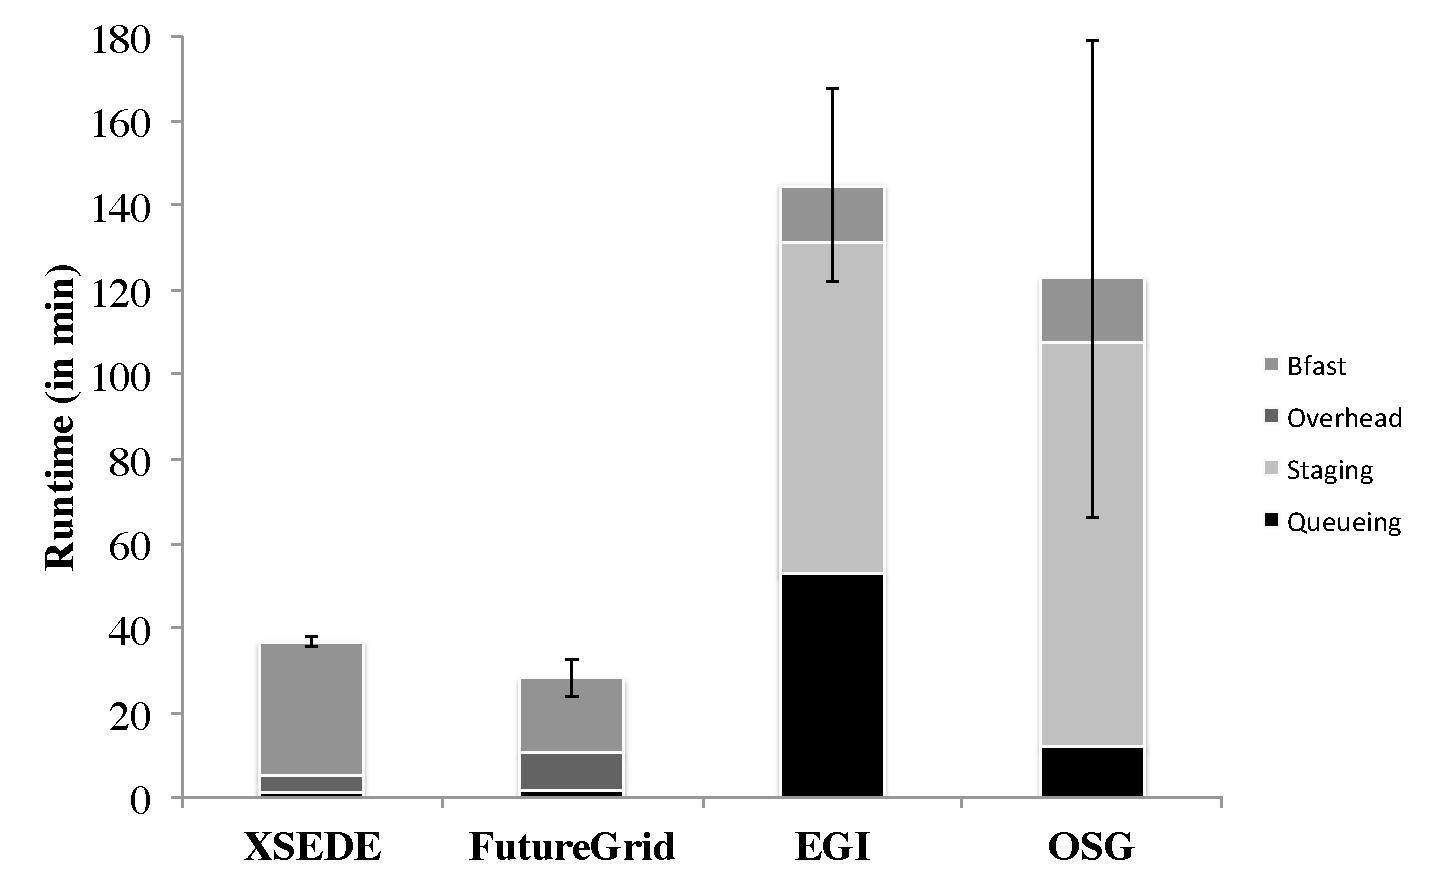
\includegraphics[width=0.48\textwidth]{../perf/interop/128-bfast-egi-fg-xsede-osg.pdf}
 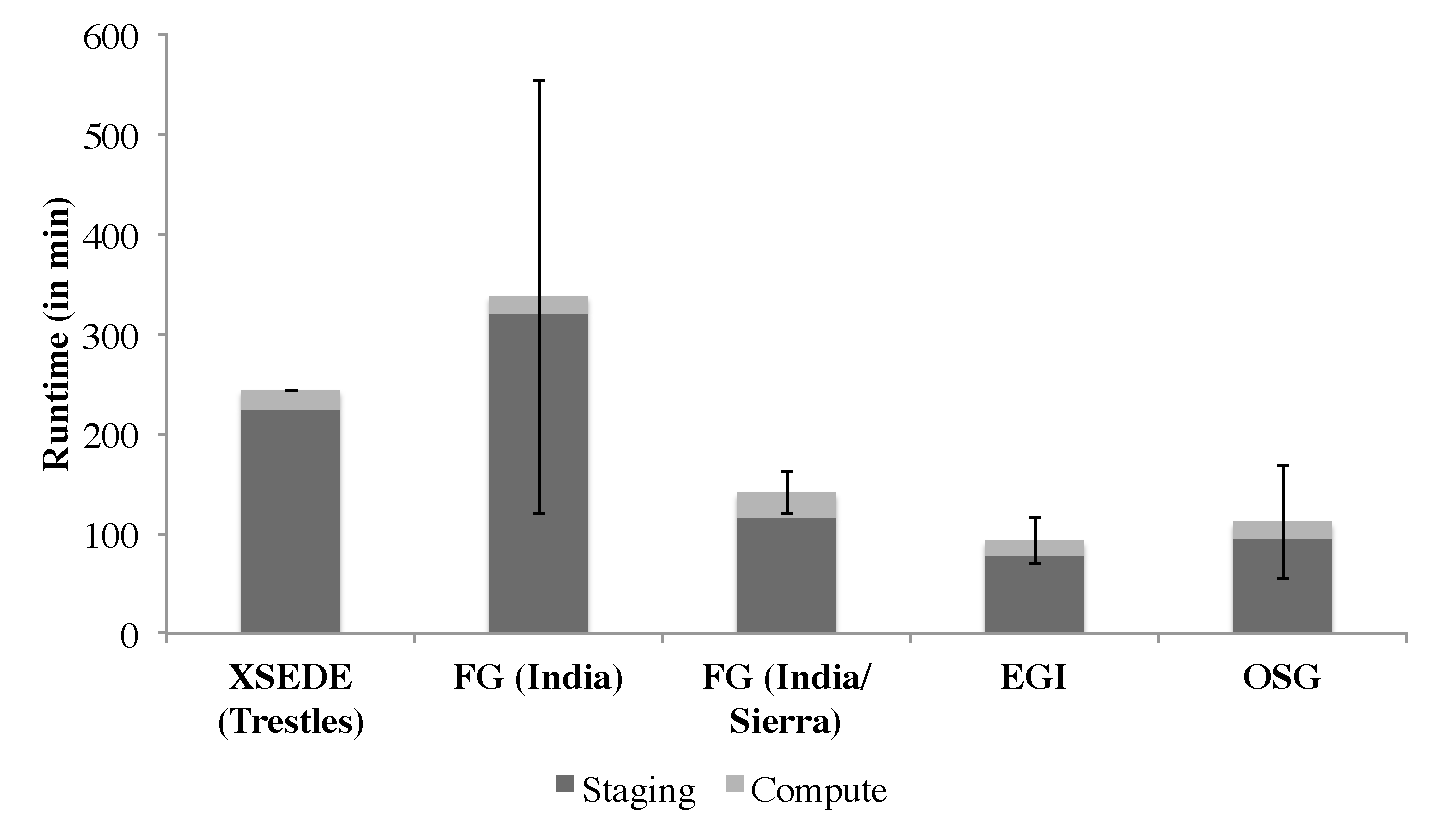
\includegraphics[width=0.48\textwidth]{../perf/interop/128-bfast-egi-fg-xsede-osg-with-staging.pdf}
 \caption{\I{\textbf{PJ Framework Performance on XSEDE, FutureGrid, EGI and 
  OSG:} Running 128 BFAST match tasks on 128 cores. Each experiment is
  repeated at least 3 times. }\up\up}
%The longer runtimes on EGI and OSG are
%  mainly caused by the longer queuing times and necessity to stage-in files.}
\label{fig:perf_perf-bfast-bj}
\end{figure}

%\jhanote{need to be consistent with case vs scenario}

\subsubsection*{Experimental Results}

Figure~\ref{fig:perf_perf-bfast-bj} shows the results of the
experiments. In addition to the runtime ($T_R$) we
measured the time to transfer input files ($T_X$), and the compute 
% \jhanote{please
%   fix!! we have runtime and actual runtime? does actual just mean
%   total runtime?} 
time $T_C$. $T_C$ also includes the overhead of
the pilot.
%which is usually ~10\,\% of the overall runtime. 
% \jhanote{I'm not sure I understand
%   this. What aspect of the pilot contributes 10\%. Why?} \alnote{I removed
% this the number since it was specific to the BJ experiments and it is
% not visible in the graphs.}

% Staging
% both
% pilot-external, i.\,e.\ queuing system (PBS, Torque, Condor) waiting
% times, as well as \pilot-internal waiting times.

% BFAST PERFORMANcE

For each \cu, the reference genome, the index files and one read file
need to be staged (1.9\,GB) -- which consumes the most significant
part of the overall runtime. In particular, on the HPC clusters, the
staging quickly becomes a bottleneck due to the fact that all \cus
share the incoming bandwidth. Also, fluctuation of the bandwidth in
this scenario leads to a high failure rate. As seen in B3 (middle
bar), the staging time can be reduced by distributing the \cus over
two machines. Generally, the performance of BFAST is heavily dependent
on the available I/O bandwidth. \jhanote{Need to have clarity between
  transfer between end-points as a bottleneck, and the I/O subsystem
  as a bottleneck. BTW what is the formal bandwidth between the two
  transfer endpoints?}

Both the index and read files need to be loaded into memory. Trestles
(XSEDE) and India/Sierra (FG) have shared network filesystems (Lustre
for Trestles, NFS for India), which are utilized by all jobs running
on these machines. The collective performance of multiple BFAST \cu
thus degrades significantly with the available I/O bandwidth, e.\,g.\
if a large number of jobs access the filesystem concurrently ( due to
the usage of NFS, the runtime on India is about 20\,\% slower than
other machines). On EGI and OSG, BFAST \cu performs best. This can
mainly be attributed to the use of local storage. \jhanote{How many
  different machines did the runs on EGI and OSG utilize? That is an
  important number to quote here} \jhanote{Also, I'm concerned that we
  are conflating staging which is IMO typically data transfer to the
  point of consumption, with 'disk I/O'}

% Queuing Time
% \alnote{to refine: queuing time not part of the diagram anymore}
% Another factor is $T_q$. In B1 and B2, $T_q$ is very low and mainly
% caused by BJ internal sub-job queueing. In B3, $T_q$ is primarily
% caused by the launch of the 128 worker agents -- each of these agents
% needs to be submitted and started via the gLite WMS; on each node, a
% DIANE worker agent must be downloaded, installed and started. In
% total, $T_q$ for each \cu was $\sim$50\,min (in cmp. $T_q$ for BJ on
% India was $\sim$9\,min). Thus, even if $T_s$ is not considered, $T_r$
% is $\sim$2.3 times longer on EGI (DIANE) than on FutureGrid (BJ).
% The
% unpredictability of $T_q$ also contributes to the higher deviation in
% $T_r$. On OSG, $T_q$ is $\sim$12 minutes, comparable to $T_q$ on
% XSEDE::Kraken.


% File Staging
% In B1 and B2, no file staging is used. On EGI and OSG resources, however, no
% shared filesystem is available; thus, files need to be transferred to the
% executing system for B3 and B4. 


% If file
% staging is not considered, OSG shows the best performance. \amnote{The amounts
% of data differ from what was stated earlier.} \amnote{The runtime should not be
% 4 to 5 times longer because of staging, if staging consumes 50\% of it -- that
% would give a factor of 2}\alnote{The runtime compared to the Kraken runtime.}




% Despite the fact that BigJob has been also installed
% with each run, it shows a significant lower startup time of 73\,sec, i.\,e.\
% about 50\,sec less than DIANE. Additionally, we also observed a runtime
% overhead of about 25\,sec for the DIANE scenario. This overhead is likely
% caused by the additional agents required. While BigJob utilizes one BJ-Agent
% on the resource, DIANE currently requires the spawning of one worker agent per
% \cu that must be executed in parallel. While the Pilot-API marshals these
% differences, i.\,e.\ while the API remains the same for both PJ frameworks, a
% light performance overhead remains observable.


% This
% can mainly be attributed to the better performance of the OSG resource, which is
% particularly visible in the BFAST runtimes, which are on average 40\,\% shorter
% than on LONI. Further, due to the lack of SAGA on OSG, BJ is deployed with the
% Redis c\&c sub-system, which shows a significantly better performance than the
% Advert Service (see section~\ref{sec:pj_performance}).

% \jhanote{What are we trying to say here?  Is it that although the API
%   is similar, semantics of implementation and execution remain
%   different, and that TROY backend handles them?}\alnote{well said}


% This part also sounds too engine-like
% Dynamic
% applications can utilize the elasticity of the TROY resource pool
% e.\,g.\ to improve the time-to-completion and/or to scale the accuracy
% of their computations.

\subsection{PJ Framework Interoperability}
\label{sec:experiment-interop}

In principal, two types of interoperability between \pilotjobs and
infrastructure exist: the first is the usage of a given PJ framework
on different infrastructures; in the scenario examined, we use BigJob
on different infrastructures in conjunction with different SAGA
adaptors. \pmnote{don't we have a interoperability at compute level; since we addressed that having same compute unit description for all infrastructures} The second is the usage of distinct PJ frameworks via the
Pilot-API, i.e., interoperability between PJ frameworks. In
configuration C1 we utilize SAGA-based interoperability by running
BigJob concurrently on FutureGrid:India and XSEDE:Trestles. C2 and C3
show PJ framework interoperability by concurrently running BigJob and
DIANE on FutureGrid:India and EGI (C2), as well as Condor and BigJob
on OSG and XSEDE:QueenBee (C3). It is worth reiterating, that to the
best of our knowledge, the latter scenario, wherein different PJ
frameworks are utilized concurrently for the same application
(whether on the same infrastructure or distinct) has never before been
realized. We attribute this to the use of the Pilot-API.  For all
scenarios, we run the same BFAST application described in
\S\ref{sec:fg-xsede-osg-egi} with 64\,\cus on each infrastructure,
i.\,e.\ in total 128\,\cus.

\begin{figure}[htbp]
  \upp
  	\centering
	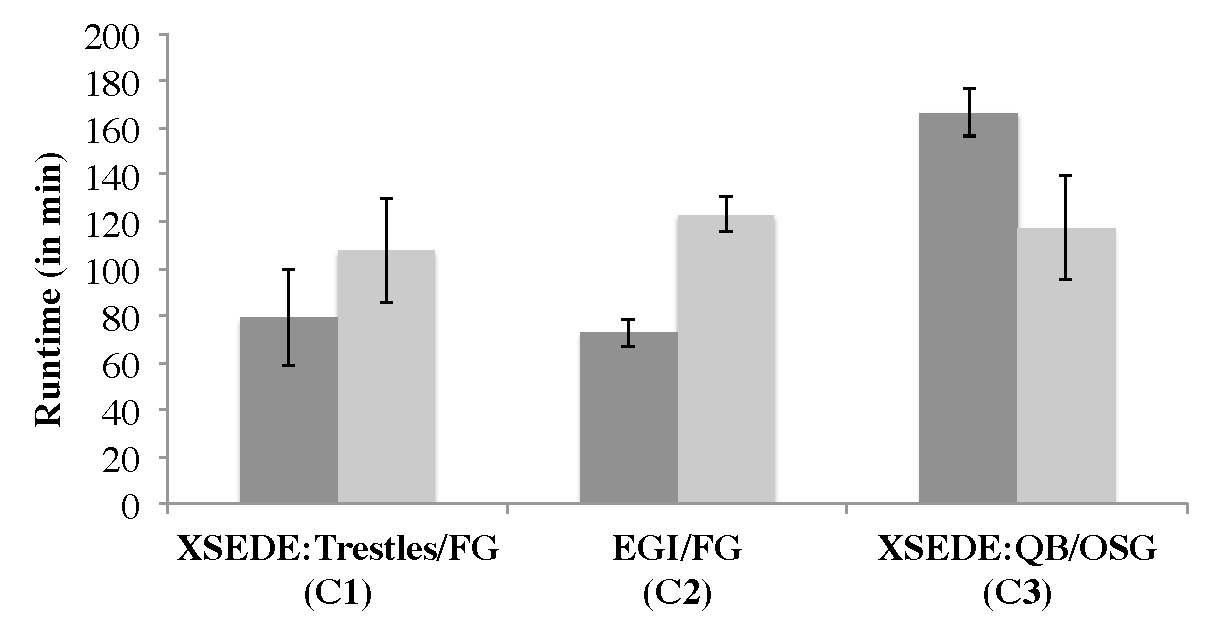
\includegraphics[width=0.48\textwidth]{../perf/interop/128-bfast-interop-with-staging.pdf}
	\caption{\I{\textbf{PJ Framework Interoperability:} Runtime of
          128 BFAST \cus on different infrastructures. \cus are
          equally distributed across the two infrastructures. The
          performance heavily depends on the available bandwidths to
          the resources, which determines the time required for file
          transfers.}}
	\label{fig:perf_interop_128-bfast-interop}
\end{figure}


Figure~\ref{fig:perf_interop_128-bfast-interop} shows the results of
the interoperability tests. In C1, one \pilot is submitted to Trestles
and one to India. 
% \jhanote{This is wrong and needs updating! I think
%   replace Kraken with Trestles. Check below for Kraken/Trestles too!} 
The overall runtime is determined by the file staging and the actual compute
time on the respective resource. Consistent with previous results the \pilot
on Trestles finished before the \pilot on India. $T_R$ of the distributed run
improved more than 50\,\% compared to a Trestles respectively the India only
run mainly due to the minimization of the incoming bandwidth bottleneck by
distributing the load to two sites.


% However, the runtime of
% the scenario is also about 20\,\% slower than running on India only.

%\jhanote{should this scenario number be different?} \alnote{sorry,
%  just moved this paragraph down from B} 

The middle bar in figure~\ref{fig:perf_interop_128-bfast-interop}
shows C2 and demonstrates that two PJ frameworks can be utilized
concurrently using the Pilot-API. As in the previous scenarios, the
overall performance heavily depends on the time required for staging
the files (for scenarios C2 and C3 we estimated the staging times
based on previous measurements). Further, some performance overhead is
induced by the distributed coordination necessary particular in case
C2 where the BJ manager is located in the EU in a high latency
environment. \jhanote{put a simple number guestimating the distributed
  coordination.. does not have to be super dooper accurate but just a
  good estimate} All communication is conducted via a Redis instance
deployed on FG, while the BJ manager is deployed on EGI; thus, for
each \cu several cross-atlantic roundtrips are necessary.
\jhanote{but still EGI finishes much faster than fG. Explain!}
Finally, C3 (right bars in
figure~\ref{fig:perf_interop_128-bfast-interop}) shows the result of
the OSG and XSEDE::QB run. Since QueenBee is an older XSEDE machine,
$T_R$ on this machine is much longer than $T_R$ on OSG despite the
necessity of file staging.

\jhanote{I think the labels of the bars
  need to change. For both C2 and C3 I think}

\subsection{Pilot-Data: Data Transfer and Management}
\label{sec:experiment-pilotdata}

\jhanote{Is it about management or is it transport we're referring
  to?}  An important challenge when running distributed data-intensive
tasks is the effective and efficient transport of data. We investigate
different data transport scenarios: (D1) the usage of
application-level file staging without PD, (D2) the usage of PD with
the SSH plugin\jhanote{what does this mean for transport}, and (D3)
the usage of PD with Globus Online. For these experiments, we utilize
Trestles (XSEDE). The input files are located on a remote machine 
(Quarry (IU) for D1; Lonestar (TACC) for D2 and D3).


\begin{figure}[t]
	\upp
	\centering
		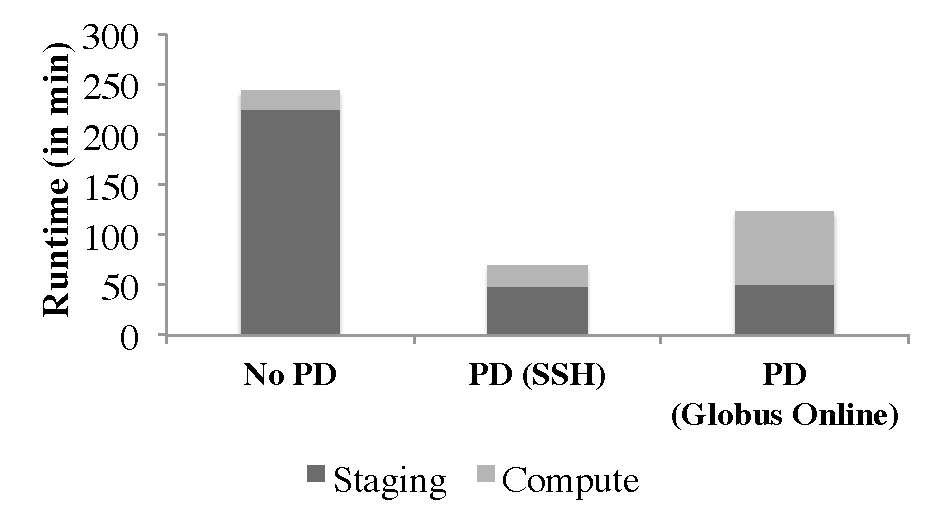
\includegraphics[width=0.4\textwidth]{../perf/sc/pd-128cus.pdf}
	\caption{\I{\textbf{Pilot-Data Performance:} Using Pilot-Data the staging 
	time can be significantly improved due to a reduction of the overall data 
	transfer volume from 128 $\cdot$ 1.9\,GB to about 24\,GB (1.9\,GB + 128 
	$\cdot$ 170\,MB). Further, Globus Online utilizes with GridFTP a more 
	efficient transfer protocol.\up\up}}
	\label{fig:perf_sc_download-concurrent-cus}
\end{figure}

\pmnote{ the dot instead of * is little bit confusing}

As previously alluded
(Figure~\ref{fig:perf_interop_128-bfast-interop}), as the number of
CUs increases, file staging quickly becomes a bottleneck, as all CUs
share the incoming bandwidth.  Also, I/O contention on the shared file
systems leads to an increasing compute time.
Figure~\ref{fig:perf_sc_download-concurrent-cus} shows that with an
increasing number of CUs, the naive way of moving files (D1) is not a
scalable solution; this is reflected in a runtime of $>$4 hours for 128
CUs.  While the download time increases linearly with the number of
CUs, the compute time remains almost constant at ~15\,min.

There are two options to address this issue: either
distribute/scale-out the computation to multiple resource (see C3), or
optimize data transfers using \pilotdata.  The optimization via
\pilotdata in turn has two components: amount transferred and transfer
protocol.  By being cognizant of the distribution of the \cus,
redundant transfers can be reduced (if not eliminated); using
\pilotdata the overall amount of data that needs to be transferred for
the 128 CU scenario can be reduced from 243\,GB (i.\,e.\ 128\,\cus
times 1.9\,GB data for the reference genome, index files and 1 read
file) to 24\,GB (a single transfer of the reference genome and index
files and 1 read file per \cu, i.\,e.\ 128 times 170\,MB ) \pmnote{This is explained in figure caption.. }.  The
staging times in D2 and D3 are comparable: both SSH and Globus Online
show some overhead compared to a plain HTTP-based transfer, but the
lower amount of data leads to a significant improvement. \jhanote{I
  don't understand how GlobusOnline has a higher overhead?} Globus
Online shows a better performance than SSH mainly due to the more
efficient GridFTP protocol.

\alnote{Add SRM discussion (time to put data, replication, ...)  data
  to large to store the complete }

% \jhanote{Where is the reason behind this explained?} \jhanote{Also, I
% can't see where B1/B2 and C1/C2 etc are defined}\alnote{Bx and Cx are defined
% in the beginning of sec B resp. C. Will do the same with configuration D.}

% \subsubsection*{BigData: A SAGA-based Pilot-Data Prototype for TROY}
\label{sec:bigdata}

\begin{figure}[t]
    \centering
    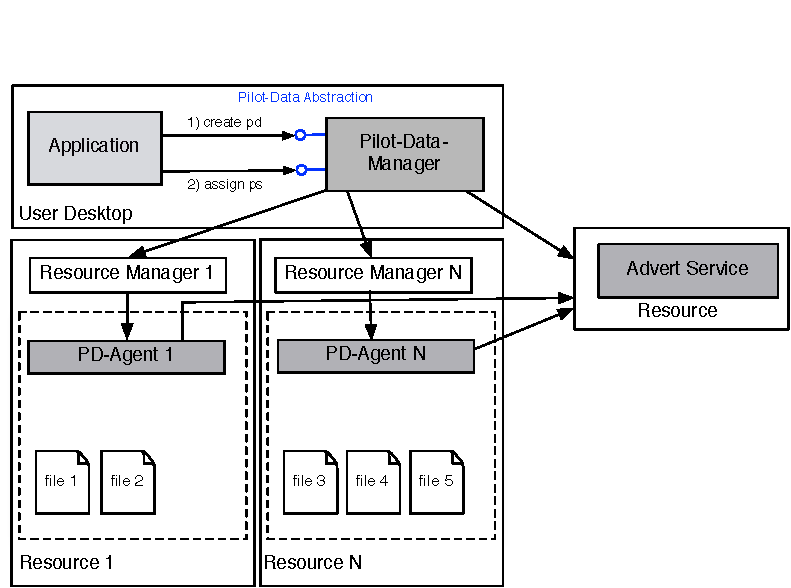
\includegraphics[width=0.48\textwidth]{figures/pilot-data-manager.pdf}
    \caption{\textbf{BigData Architecture:} The BD Manager exposes
      TROY's PD API. Application can create group of files and assign
      files to storage. The BD manager tracks file locations in the
      data catalog. The scheduler optimizes data-compute co-location.
      The transfer manager initiates and monitors data
      movements. \up\up}
    \label{fig:pilot-data-architecture}
\end{figure}

% \begin{figure*}[t]
%   \up\up\up
%   \begin{minipage}[t]{0.475\linewidth}
%     \centering
%     \includegraphics[width=\textwidth]{figures/distributed_pilot_job.pdf}
%     %\includegraphics[width=\textwidth]{figures/P1140340.JPG}
%     \caption{\textbf{BigJob -- SAGA-based Pilot-Job Implementation:}
%       BigJob is the implementation of the actual PJ functionality for
%       TROY. SAGA BigJob permits usage with multiple middleware
%       backends~\cite{}}
%     \label{fig:figures_distributed_pilot_job}
%     \end{minipage}
%   \hspace{0.035\linewidth}
%   \begin{minipage}[t]{0.475\linewidth}
%     \centering
%     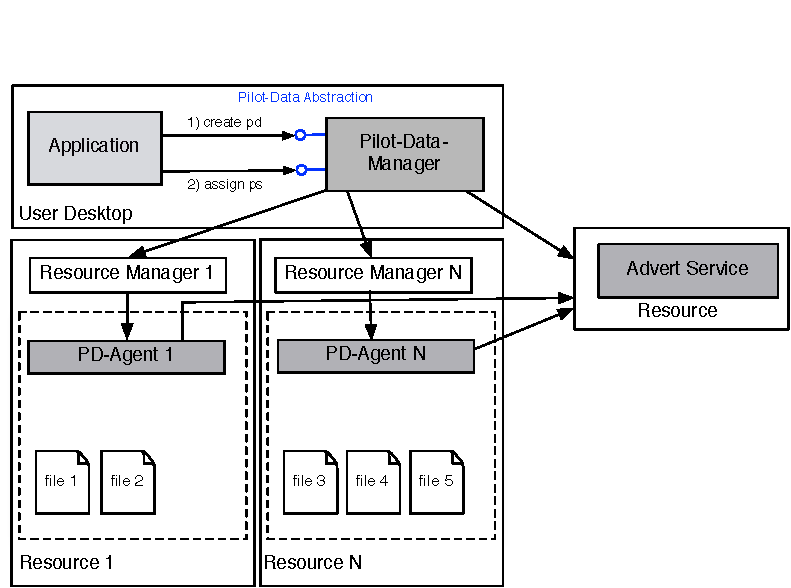
\includegraphics[width=\textwidth]{figures/pilot-data-manager.pdf}
%     \caption{\textbf{BigData Architecture:} The BD Manager exposes
%       TROY's PD API. Application can create group of files and assign 
%       files to storage. The BD manager tracks file locations in
%       the data catalog. The scheduler optimizes data-compute co-location.
%       The transfer manager initiates and monitors data movements. \up\up}
%     \label{fig:pilot-data-architecture}
%     \end{minipage}
% \end{figure*}

BigData-SAGA is the SAGA-based prototype of the Pilot-Data
abstraction; in the scope of this paper it is referred to as simply
BigData (BD).  Figure~\ref{fig:pilot-data-architecture} gives an
overview of the architecture.  The system consists of two components:
the BD manager, and the BD agents deployed on the physical
resources. The coordination scheme used is again M/W with some
intelligence that is located de-centrally at the BD agent. As
communication mechanism the SAGA Advert Service is used, in a similar
push/pull mode as for BJ.

The BD manager is responsible for 1) meta-data management, i.\,e.\ it
keeps track of the pilot stores that a pilot data object is associated
with, 2) for scheduling data movements and data replications (taking
into account the application requirements defined via affinities), and
3) for managing data movements activities.  Similar to BigJob, an
agent on each resource is used to manage the physical storage on a
resource.  

A particular critical requirement for data-intensive application, is
the management of affinity between DUs and also between WUs and
DUs. The BD scheduler supports preliminary affinity-aware
scheduling: both BigJob and BigData are tightly integrated to
efficiently support compute- and data-related aspects of dynamic
execution (see also \S{IIIA}).
 
\jhanote{Andre, please review the next paragraph: Should it just go
  for simplicity?} Thus, Pilot-Data introduces the PD container object
for expressing relationships between DUs. A PD corresponds to an SU in
the P* Model, i.\,e.\ it is used as scheduling unit for internal
optimizations, e.\,g.\ the grouping of DUs. Having instantiated a PD,
it can be assigned to a PS via the PD manager. A PS is a placeholder
reserving a certain amount of storage, i.\,e.\ it corresponds to a
pilot in the pilot-job model. By associating a PD to a PS the data is
actually moved to the physical location associated with the PS. The PD
manager facilitates the creation of PSs, schedules data movements
(with respect to specified affinities) and manages data accesses.


%%%%%%%%%%%%%%%%%%%%%%%%%%%%%%%%%%%%%%%%%%%%%%%%%%%%%%%%%%%%%%%%%%%%%%


% In addition to the three Pilot-Job framework discussed in this section, various
% other frameworks exist.
% \begin{itemize}
%     \item MyCluster~\cite{1652061} enables the 
% creation of a Condor, PBS or SGE clusters on-demand.
%     \item Falkon~\cite{1362680} is a Pilot-Job framework that emphasizes the 
% performance of its task dispatcher.
%     \item Nimrod/G~\cite{10.1109/HPC.2000.846563}
%     \item DIRAC~\cite{1742-6596-219-6-062049} is another pilot-job framework 
% used by the LHCb community.
%     \item ToPoS~\cite{topos} is a REST-based web service primarily designed with 
% respect to parameter sweep applications. Internally, ToPoS utilizes PJ 
% capabilities to efficiently manage resources.
%     \item The Production and Distributed Analysis System 
% (PanDA)~\cite{1742-6596-219-6-062041} is the workload management system of 
% the ATLAS experiment. PanDA utilizes multi-user PJs for resource management. 
% The PJ component is built on top of Condor-G and referred to as AutoPilot. 
% It can also be used independently of the ATLAS environment. 
% \end{itemize}


% 
% Both BigJob and BigData define similar elements that can be mapped to
% each other. Nevertheless, compute and data model sometimes require a
% different treatment.  The extended TROY (an implementation of the
% extended P* Model) will optimize data- and computing according to a
% set of defined affinities and policies.

% BJ and BD encapsulate cross-cutting properties across data and
% computation. 

% With the maturing of both models and
% implementations, we expect that both the PJ and PD model converge in
% the future.

\section{Discussion and Future Work}
\label{sec:discussion-future-work}

% \jhanote{This will probably have to go due to space: In summary, the
%   Pilot-API enables applications to utilize a dynamic resource pool
%   consisting of resources of different infrastructures, e.\,g.\ EGI
%   and FutureGrid, but also XSEDE resources, at large-scales hitherto
%   unattainable.}

% \note{Future Work: optimizations (parallel queuing and transferring)}

The primary intellectual contribution of this work has been the
development of the P* Model -- a common abstract model for describing
and characterizing Pilot-abstractions, the mapping of P* elements to
PJ frameworks such as DIANE and Condor-G/Glide-in and the design and
development of the Pilot-API -- that reflects the P* elements and
characteristics.  We validate the P* Model by demonstrating that the
most widely used PJ frameworks, viz., DIANE and Condor-G/Glide-in can
be compared, contrasted and analyzed using this analytical framework.
Furthermore we demonstrate the use of the Pilot-API -- which provides
a common access layer to different PJ frameworks, with multiple PJ
frameworks over distributed production cyberinfrastructure, such as
XSEDE, OSG, EGI and FutureGrid. 

The Pilot-API does not represent a barrier to scalability, but
provides the ability to overcome scalability limitations of certain
infrastructure caused e.\,g.\ by I/O, memory, and/or bandwidth
bottlenecks, via the usage of a diverse set of distributed,
heterogeneous infrastructures via a unified API.  Although the aim of
our experiments is the demonstration of the interoperable use of
hitherto distinct and disjoint \pilotjobs, in the process we highlight
the performance advantages that can emanate from the ability to
seamlessly distribute (I/O intensive) workloads in a scalable manner.
While scale-out introduces some overheads (e.\,g.\ in particular for
data-intensive applications, large amounts data need to be moved), it
enables application to improve performance, e.\,g.\ by offloading
parts of the computation to a faster resource (see C1), and to scale
its problem set, e.\,g.\ by utilizing more resources at the same time.
P* provides significant future development, research \& deployment
opportunities, for example, explore and reason on the relative roles
of system versus application-level scheduling, heuristics for dynamic
execution and the role of affinity.  


% \jhanote{Ole: Please Please Please put down an analysis of why an API
%   is not enough and the deployment challenges that remain. In other
%   words, the API is a necessary starting point, but not a sufficient
%   point.}

% \onote{Merged from above... not sure what do do with this: As we will
%   see further in \S V (Experiments), 

% Native infrastructure refers to the infrastructure for
% which a PJ framework has been primarily developed for and on which
% infrastructures it is mainly used,
% that does not mean, however, that these frameworks do not work on
% other infrastructures.}

The Pilot-API is being deployed to support production-scale science on
production infrastructure (as demonstrated by the emphasis on
production infrastructure in our experimentation).
However, attention to several deployment issues will be required in
order to realize the full power of the P* Model.  For example, in
spite of a common Pilot-API each PJ framework has a rather different
usage modality; this is reflective of the fact that typically, PJ
frameworks ``evolve in'' and are ``native to'' specific e.g.,
Condor-G/Glide-in is the native PJ framework of the Open Science Grid
and its use is heavily coupled with WMS infrastructure.  Additionally,
our experience with fragile grid middleware and infrastructures has
taught us to appreciate the significance of the ease of deployment and
the need for robustness of tools and software on heterogeneous
distributed infrastructures.

Our fundamental research has immense practical implications and
potential: Although current PJ frameworks collectively support
millions of tasks yearly on several production distributed
infrastructure, extensibility and interoperability remain significant
challenges~\cite{extenci}.  Given the increasing importance of
\pilotjobs and the challenges associated with distributed data
placement, our work which provides both a conceptual model and
practical solutions has the potential to improve this situation.  In
fact, it is a stated goal of our research to enhance the range of
applications and usage-modes that will benefit from the \pilot
abstraction, by deeply integrating Pilot-API/P* capabilities with
multiple production infrastructures~\cite{bigjob_web}.


% The P* model was used to demonstrate We established PJ and PD as
% abstractions for supporting dynamic execution by decoupling workload
% and resource assignment/scheduling.

% they share different important properties with respect to the commonly
% used communication and coordination schemes.

% \alnote{Add discussion on limitations of API - address these
%   limitations in a common runtime system.}


% The P* Model provides a common abstract model for describing and
% characterizing Pilot-abstractions.  
% The Pilot-API also enables the concurrent use of multiple PJ
% frameworks, thus providing interoperability and extensibility.

% By using the capabilities of the Pilot-API, i.\,e.\ the decoupling
% of workload submission from resource assignment, applications can
% scale-out on multiple and possibly heterogeneous resources in a
% flexible way.

% \jhanote{merge this with above paragraph} In summary, the Pilot-API
% enables the usage of a diverse set of distributed, heterogeneous
% infrastructures via a unified API. As shown, the Pilot-API does not
% represent a barrier to scalability, but provides the ability to
% overcome scalability limitations of certain infrastructure caused
% e.\,g.\ by I/O, memory, and/or bandwidth bottlenecks. By using the
% capabilities of the Pilot-API, i.\,e.\ the decoupling of workload
% submission from resource assignment, applications can scale-out on
% multiple and possibly heterogeneous resources in a flexible
% way. While scale-out introduces some overheads (e.\,g.\ in
% particular for data-intensive applications, large amounts data need
% to be moved), it enables application to improve performance, e.\,g.\
% by offloading parts of the computation to a faster resource (see
% C1), and to scale its problem set, e.\,g.\ by utilizing more
% resources at the same time.

%The Pilot-API reflects the P* elements and characteristics, and
%provides a common access layer to different PJ framewors via a uniform
%API; 

% , i.\,e.\ the architecture and the communication and coordination
% schemes.\alnote{i.e. sub-clause can go} .  Building on the P* Model,
% the Pilot-API's design enables the easy exchange of PJ
% implementations, and also The Pilot-API functions as common access
% layer for different PJ frameworks, thus


% However, the SAGA inspired approach to the Pilot-API design and the
% leverage of the design and deployment experiences of SAGA, e.\,g.\ by
% moving the responsibility of correctly deployed grid-middleware to the
% resource providers and not the end-users, should be an effective
% solution. 


% We discuss one opportunity along each of these axes:
% (i) Development and Extension: In order to overcome limitations of the
% API-based approach we will develop a complete implementation of the P*
% Model -- called TROY (Tiered Resource Overlay). TROY will provide
% deeper integration of the Pilot-API via a semantic mapping of the P*
% elements and characteristics to \pilotjob frameworks.  TROY will also
% provide a unified -- compute and data, implementation of P*, e.g.,
% BigData analogous to BigJob; (ii) Research Issues: 
%These developments and extensions will also provide


% TROY -- which embodies the P*
% Model, is being designed with usability, reliability and robustness as
% first-class considerations.

% On the basis of successful validation of the P* Model, we propose
% extensions to include data.  For example, presenting unified
% abstractions within the Pilot-API and

% Additionally we aim to provide explicit support for advanced dynamic
% execution modes and 

% In summary, we will use existing and emerging capabilities of TROY to
% support the efficient and scalable solution of many scientific
% applications that involve multiple independent tasks.\alnote{just one sentence - can be merged with paragraph above.}

% It is not possible to anticipate all of the tools and abstractions
% that distributed applications will need down the road. Changes in
% infrastructure and application requirements cannot be predicted. For
% this reason, tools must provide open interfaces to enable more easy
% integration and interoperation with other tools. Whether this can be
% best achieved by new extensible tools or “tool orchestration” or a
% tool “framework” is an open question. This, of course, does not
% preclude the internal evolution of existing tools to implement new
% abstractions, but just this is not enough in our view.

%\up
\section*{Acknowledgements}
%\up
\footnotesize \footnotesize{This work is funded by NSF CHE-1125332
  (Cyber-enabled Discovery and Innovation), HPCOPS NSF-OCI 0710874
  award, NSF-ExTENCI (OCI-1007115) and NIH Grant Number P20RR016456
  from the NIH National Center For Research Resources. Important
  funding for SAGA has been provided by the UK EPSRC grant number
  GR/D0766171/1 (via OMII-UK) and the Cybertools project (PI Jha)
  NSF/LEQSF (2007-10)-CyberRII-01, NSF EPSCoR Cooperative Agreement
  No. EPS-1003897 with additional support from the Louisiana Board of
  Regents.  SJ acknowledges the e-Science Institute, Edinburgh for
  supporting the research theme. ``Distributed Programming
  Abstractions'' \& 3DPAS. MS is sponsored by the program of BiG Grid,
  the Dutch e-Science Grid, which is financially supported by the
  Netherlands Organisation for Scientific Research, NWO. SJ
  acknowledges useful related discussions with Jon Weissman
  (Minnesota) and Dan Katz (Chicago). We thank J Kim (CCT) for
  assistance with BFAST.  This work has also been made possible thanks
  to computer resources provided by TeraGrid TRAC award TG-MCB090174
  (Jha) and BiG Grid.  This document was developed with support from
  the US NSF under Grant No. 0910812 to Indiana University for
  ``FutureGrid: An Experimental, High-Performance Grid Test-bed''.}

  
%\bibliographystyle{plain}
%\bibliographystyle{IEEEtranS}
\bibliographystyle{IEEEtran}
\bibliography{../pilotjob,../saga,../saga-related}


\end{document}

